\documentclass[twoside]{book}

% Packages required by doxygen
\usepackage{fixltx2e}
\usepackage{calc}
\usepackage{doxygen}
\usepackage[export]{adjustbox} % also loads graphicx
\usepackage{graphicx}
\usepackage[utf8]{inputenc}
\usepackage{makeidx}
\usepackage{multicol}
\usepackage{multirow}
\PassOptionsToPackage{warn}{textcomp}
\usepackage{textcomp}
\usepackage[nointegrals]{wasysym}
\usepackage[table]{xcolor}

% Font selection
\usepackage[T1]{fontenc}
\usepackage[scaled=.90]{helvet}
\usepackage{courier}
\usepackage{amssymb}
\usepackage{sectsty}
\renewcommand{\familydefault}{\sfdefault}
\allsectionsfont{%
  \fontseries{bc}\selectfont%
  \color{darkgray}%
}
\renewcommand{\DoxyLabelFont}{%
  \fontseries{bc}\selectfont%
  \color{darkgray}%
}
\newcommand{\+}{\discretionary{\mbox{\scriptsize$\hookleftarrow$}}{}{}}

% Page & text layout
\usepackage{geometry}
\geometry{%
  a4paper,%
  top=2.5cm,%
  bottom=2.5cm,%
  left=2.5cm,%
  right=2.5cm%
}
\tolerance=750
\hfuzz=15pt
\hbadness=750
\setlength{\emergencystretch}{15pt}
\setlength{\parindent}{0cm}
\setlength{\parskip}{3ex plus 2ex minus 2ex}
\makeatletter
\renewcommand{\paragraph}{%
  \@startsection{paragraph}{4}{0ex}{-1.0ex}{1.0ex}{%
    \normalfont\normalsize\bfseries\SS@parafont%
  }%
}
\renewcommand{\subparagraph}{%
  \@startsection{subparagraph}{5}{0ex}{-1.0ex}{1.0ex}{%
    \normalfont\normalsize\bfseries\SS@subparafont%
  }%
}
\makeatother

% Headers & footers
\usepackage{fancyhdr}
\pagestyle{fancyplain}
\fancyhead[LE]{\fancyplain{}{\bfseries\thepage}}
\fancyhead[CE]{\fancyplain{}{}}
\fancyhead[RE]{\fancyplain{}{\bfseries\leftmark}}
\fancyhead[LO]{\fancyplain{}{\bfseries\rightmark}}
\fancyhead[CO]{\fancyplain{}{}}
\fancyhead[RO]{\fancyplain{}{\bfseries\thepage}}
\fancyfoot[LE]{\fancyplain{}{}}
\fancyfoot[CE]{\fancyplain{}{}}
\fancyfoot[RE]{\fancyplain{}{\bfseries\scriptsize Generated by Doxygen }}
\fancyfoot[LO]{\fancyplain{}{\bfseries\scriptsize Generated by Doxygen }}
\fancyfoot[CO]{\fancyplain{}{}}
\fancyfoot[RO]{\fancyplain{}{}}
\renewcommand{\footrulewidth}{0.4pt}
\renewcommand{\chaptermark}[1]{%
  \markboth{#1}{}%
}
\renewcommand{\sectionmark}[1]{%
  \markright{\thesection\ #1}%
}

% Indices & bibliography
\usepackage{natbib}
\usepackage[titles]{tocloft}
\setcounter{tocdepth}{3}
\setcounter{secnumdepth}{5}
\makeindex

% Hyperlinks (required, but should be loaded last)
\usepackage{ifpdf}
\ifpdf
  \usepackage[pdftex,pagebackref=true]{hyperref}
\else
  \usepackage[ps2pdf,pagebackref=true]{hyperref}
\fi
\hypersetup{%
  colorlinks=true,%
  linkcolor=blue,%
  citecolor=blue,%
  unicode%
}

% Custom commands
\newcommand{\clearemptydoublepage}{%
  \newpage{\pagestyle{empty}\cleardoublepage}%
}

\usepackage{caption}
\captionsetup{labelsep=space,justification=centering,font={bf},singlelinecheck=off,skip=4pt,position=top}

%===== C O N T E N T S =====

\begin{document}

% Titlepage & ToC
\hypersetup{pageanchor=false,
             bookmarksnumbered=true,
             pdfencoding=unicode
            }
\pagenumbering{alph}
\begin{titlepage}
\vspace*{7cm}
\begin{center}%
{\Large Easyuino \\[1ex]\large 1.\+2.\+0 }\\
\vspace*{1cm}
{\large Generated by Doxygen 1.8.13}\\
\end{center}
\end{titlepage}
\clearemptydoublepage
\pagenumbering{roman}
\tableofcontents
\clearemptydoublepage
\pagenumbering{arabic}
\hypersetup{pageanchor=true}

%--- Begin generated contents ---
\chapter{Hierarchical Index}
\section{Class Hierarchy}
This inheritance list is sorted roughly, but not completely, alphabetically\+:\begin{DoxyCompactList}
\item \contentsline{section}{Easyuino\+:\+:Device}{\pageref{class_easyuino_1_1_device}}{}
\begin{DoxyCompactList}
\item \contentsline{section}{Easyuino\+:\+:Distance\+Meter}{\pageref{class_easyuino_1_1_distance_meter}}{}
\begin{DoxyCompactList}
\item \contentsline{section}{Easyuino\+:\+:Distance\+Meter\+Non\+Block}{\pageref{class_easyuino_1_1_distance_meter_non_block}}{}
\begin{DoxyCompactList}
\item \contentsline{section}{Easyuino\+:\+:Distance\+Meter\+Accurate}{\pageref{class_easyuino_1_1_distance_meter_accurate}}{}
\end{DoxyCompactList}
\item \contentsline{section}{Easyuino\+:\+:Distance\+Meter\+Printable}{\pageref{class_easyuino_1_1_distance_meter_printable}}{}
\end{DoxyCompactList}
\item \contentsline{section}{Easyuino\+:\+:G\+S\+M\+Service}{\pageref{class_easyuino_1_1_g_s_m_service}}{}
\begin{DoxyCompactList}
\item \contentsline{section}{Easyuino\+:\+:G\+S\+M\+Service\+Secure}{\pageref{class_easyuino_1_1_g_s_m_service_secure}}{}
\end{DoxyCompactList}
\item \contentsline{section}{Easyuino\+:\+:Infra\+Red\+Receiver}{\pageref{class_easyuino_1_1_infra_red_receiver}}{}
\item \contentsline{section}{Easyuino\+:\+:Relay}{\pageref{class_easyuino_1_1_relay}}{}
\begin{DoxyCompactList}
\item \contentsline{section}{Easyuino\+:\+:Relay\+Named}{\pageref{class_easyuino_1_1_relay_named}}{}
\end{DoxyCompactList}
\item \contentsline{section}{Easyuino\+:\+:R\+G\+B\+Led}{\pageref{class_easyuino_1_1_r_g_b_led}}{}
\item \contentsline{section}{Easyuino\+:\+:Seven\+Segments}{\pageref{class_easyuino_1_1_seven_segments}}{}
\item \contentsline{section}{Easyuino\+:\+:Water\+Detector}{\pageref{class_easyuino_1_1_water_detector}}{}
\item \contentsline{section}{Easyuino\+:\+:Water\+Flow\+Sensor}{\pageref{class_easyuino_1_1_water_flow_sensor}}{}
\begin{DoxyCompactList}
\item \contentsline{section}{Easyuino\+:\+:Water\+Flow\+Meter}{\pageref{class_easyuino_1_1_water_flow_meter}}{}
\end{DoxyCompactList}
\end{DoxyCompactList}
\item \contentsline{section}{Manual\+Test}{\pageref{class_manual_test}}{}
\begin{DoxyCompactList}
\item \contentsline{section}{Distance\+Meter\+Accurate\+Test}{\pageref{class_distance_meter_accurate_test}}{}
\item \contentsline{section}{Distance\+Meter\+Non\+Block\+Test}{\pageref{class_distance_meter_non_block_test}}{}
\item \contentsline{section}{Distance\+Meter\+Test}{\pageref{class_distance_meter_test}}{}
\item \contentsline{section}{Relay\+Named\+Test}{\pageref{class_relay_named_test}}{}
\item \contentsline{section}{Relay\+Test}{\pageref{class_relay_test}}{}
\item \contentsline{section}{R\+G\+B\+Led\+Test}{\pageref{class_r_g_b_led_test}}{}
\item \contentsline{section}{Water\+Detector\+Test}{\pageref{class_water_detector_test}}{}
\end{DoxyCompactList}
\item \contentsline{section}{Easyuino\+:\+:Printable}{\pageref{class_easyuino_1_1_printable}}{}
\begin{DoxyCompactList}
\item \contentsline{section}{Easyuino\+:\+:Distance\+Meter\+Printable}{\pageref{class_easyuino_1_1_distance_meter_printable}}{}
\item \contentsline{section}{Easyuino\+:\+:Relay\+Named}{\pageref{class_easyuino_1_1_relay_named}}{}
\end{DoxyCompactList}
\item \contentsline{section}{Easyuino\+:\+:S\+MS}{\pageref{class_easyuino_1_1_s_m_s}}{}
\item \contentsline{section}{Easyuino\+:\+:Utilities}{\pageref{class_easyuino_1_1_utilities}}{}
\end{DoxyCompactList}

\chapter{Class Index}
\section{Class List}
Here are the classes, structs, unions and interfaces with brief descriptions\+:\begin{DoxyCompactList}
\item\contentsline{section}{\hyperlink{class_easyuino_1_1_button}{Easyuino\+::\+Button} \\*\hyperlink{class_easyuino_1_1_button}{Button} A\+PI offers an interface to interact with common buttons }{\pageref{class_easyuino_1_1_button}}{}
\item\contentsline{section}{\hyperlink{class_easyuino_1_1_device}{Easyuino\+::\+Device} \\*General class that provides the common A\+PI behaviour for all the devices/sensors }{\pageref{class_easyuino_1_1_device}}{}
\item\contentsline{section}{\hyperlink{class_easyuino_1_1_distance_meter}{Easyuino\+::\+Distance\+Meter} \\*Used to represent the at least supported Ultrasonic Module models enum Ultrasonic\+Module \+: uint8\+\_\+t \{ H\+C\+\_\+\+S\+R03, H\+C\+\_\+\+S\+R04, H\+C\+\_\+\+S\+R05 \}; }{\pageref{class_easyuino_1_1_distance_meter}}{}
\item\contentsline{section}{\hyperlink{class_easyuino_1_1_distance_meter_accurate}{Easyuino\+::\+Distance\+Meter\+Accurate} \\*\hyperlink{class_easyuino_1_1_distance_meter_accurate}{Distance\+Meter\+Accurate} offers an A\+PI to interact with an Ultrasonic Module to measure distances considering the current air temperature (due to the effect that the air temperature have in the sound speed in air) }{\pageref{class_easyuino_1_1_distance_meter_accurate}}{}
\item\contentsline{section}{\hyperlink{class_easyuino_1_1_distance_meter_non_block}{Easyuino\+::\+Distance\+Meter\+Non\+Block} \\*\hyperlink{class_easyuino_1_1_distance_meter_non_block}{Distance\+Meter\+Non\+Block} offers an A\+PI to interact with an Ultrasonic Module to measure distance in a non-\/block way }{\pageref{class_easyuino_1_1_distance_meter_non_block}}{}
\item\contentsline{section}{\hyperlink{class_easyuino_1_1_distance_meter_printable}{Easyuino\+::\+Distance\+Meter\+Printable} \\*It offers the same A\+PI as \hyperlink{class_easyuino_1_1_distance_meter}{Distance\+Meter} plus some methods to print the internal state into a stream for example }{\pageref{class_easyuino_1_1_distance_meter_printable}}{}
\item\contentsline{section}{\hyperlink{class_easyuino_1_1_g_s_m_service}{Easyuino\+::\+G\+S\+M\+Service} \\*\hyperlink{class_easyuino_1_1_g_s_m_service}{G\+S\+M\+Service} A\+PI allows to interact with G\+SM boards in order to perform calls, sms management etc }{\pageref{class_easyuino_1_1_g_s_m_service}}{}
\item\contentsline{section}{\hyperlink{class_easyuino_1_1_g_s_m_service_secure}{Easyuino\+::\+G\+S\+M\+Service\+Secure} \\*\hyperlink{class_easyuino_1_1_g_s_m_service_secure}{G\+S\+M\+Service\+Secure} extends the \hyperlink{class_easyuino_1_1_g_s_m_service}{G\+S\+M\+Service} A\+PI allowing user to add phone numbers to accept calls and S\+M\+Ss from this predefined set of numbers }{\pageref{class_easyuino_1_1_g_s_m_service_secure}}{}
\item\contentsline{section}{\hyperlink{class_easyuino_1_1_infra_red_receiver}{Easyuino\+::\+Infra\+Red\+Receiver} }{\pageref{class_easyuino_1_1_infra_red_receiver}}{}
\item\contentsline{section}{\hyperlink{class_easyuino_1_1_printable}{Easyuino\+::\+Printable} \\*Provides an interface interface to write objects to a Stream }{\pageref{class_easyuino_1_1_printable}}{}
\item\contentsline{section}{\hyperlink{class_easyuino_1_1_relay}{Easyuino\+::\+Relay} \\*\hyperlink{class_easyuino_1_1_relay}{Relay} offers a simple A\+PI to interact with relay devices }{\pageref{class_easyuino_1_1_relay}}{}
\item\contentsline{section}{\hyperlink{class_easyuino_1_1_relay_named}{Easyuino\+::\+Relay\+Named} \\*\hyperlink{class_easyuino_1_1_relay_named}{Relay\+Named} offers the same A\+PI of the \hyperlink{class_easyuino_1_1_relay}{Relay} plus the possibility to associate a string label to the A\+PI object }{\pageref{class_easyuino_1_1_relay_named}}{}
\item\contentsline{section}{\hyperlink{class_easyuino_1_1_r_g_b_led}{Easyuino\+::\+R\+G\+B\+Led} \\*\hyperlink{class_easyuino_1_1_r_g_b_led}{R\+G\+B\+Led} A\+PI allows to easily interact with a R\+GB led to set its color for example }{\pageref{class_easyuino_1_1_r_g_b_led}}{}
\item\contentsline{section}{\hyperlink{class_easyuino_1_1_seven_segments}{Easyuino\+::\+Seven\+Segments} \\*\hyperlink{class_easyuino_1_1_seven_segments}{Seven\+Segments} A\+PI is used to interact with seven segments displays }{\pageref{class_easyuino_1_1_seven_segments}}{}
\item\contentsline{section}{\hyperlink{class_easyuino_1_1_s_m_s}{Easyuino\+::\+S\+MS} \\*Represents a \hyperlink{class_easyuino_1_1_s_m_s}{S\+MS} object used to send and receive it from the \hyperlink{class_easyuino_1_1_g_s_m_service}{G\+S\+M\+Service} A\+PI }{\pageref{class_easyuino_1_1_s_m_s}}{}
\item\contentsline{section}{\hyperlink{class_easyuino_1_1_utilities}{Easyuino\+::\+Utilities} \\*Provides some auxiliary functions for internal use in library but at same time expose it to public for the library users }{\pageref{class_easyuino_1_1_utilities}}{}
\item\contentsline{section}{\hyperlink{class_easyuino_1_1_water_detector}{Easyuino\+::\+Water\+Detector} \\*Rain\+Detector A\+PI is used to detect the amount of water that is touching the sensor }{\pageref{class_easyuino_1_1_water_detector}}{}
\item\contentsline{section}{\hyperlink{class_easyuino_1_1_water_flow_meter}{Easyuino\+::\+Water\+Flow\+Meter} \\*\hyperlink{class_easyuino_1_1_water_flow_meter}{Water\+Flow\+Meter} A\+PI extends the \hyperlink{class_easyuino_1_1_water_flow_sensor}{Water\+Flow\+Sensor} A\+PI adding the possiblity to know how much water is flowing and how much have flown in total }{\pageref{class_easyuino_1_1_water_flow_meter}}{}
\item\contentsline{section}{\hyperlink{class_easyuino_1_1_water_flow_sensor}{Easyuino\+::\+Water\+Flow\+Sensor} \\*\hyperlink{class_easyuino_1_1_water_flow_sensor}{Water\+Flow\+Sensor} is an A\+PI offers the ability to know if it is flowing something through the sensor or not using fluid flow meters }{\pageref{class_easyuino_1_1_water_flow_sensor}}{}
\end{DoxyCompactList}

\chapter{Class Documentation}
\hypertarget{class_easyuino_1_1_button}{}\section{Easyuino\+:\+:Button Class Reference}
\label{class_easyuino_1_1_button}\index{Easyuino\+::\+Button@{Easyuino\+::\+Button}}


\hyperlink{class_easyuino_1_1_button}{Button} A\+PI offers an interface to interact with common buttons.  




{\ttfamily \#include $<$Button.\+h$>$}

Inheritance diagram for Easyuino\+:\+:Button\+:\begin{figure}[H]
\begin{center}
\leavevmode
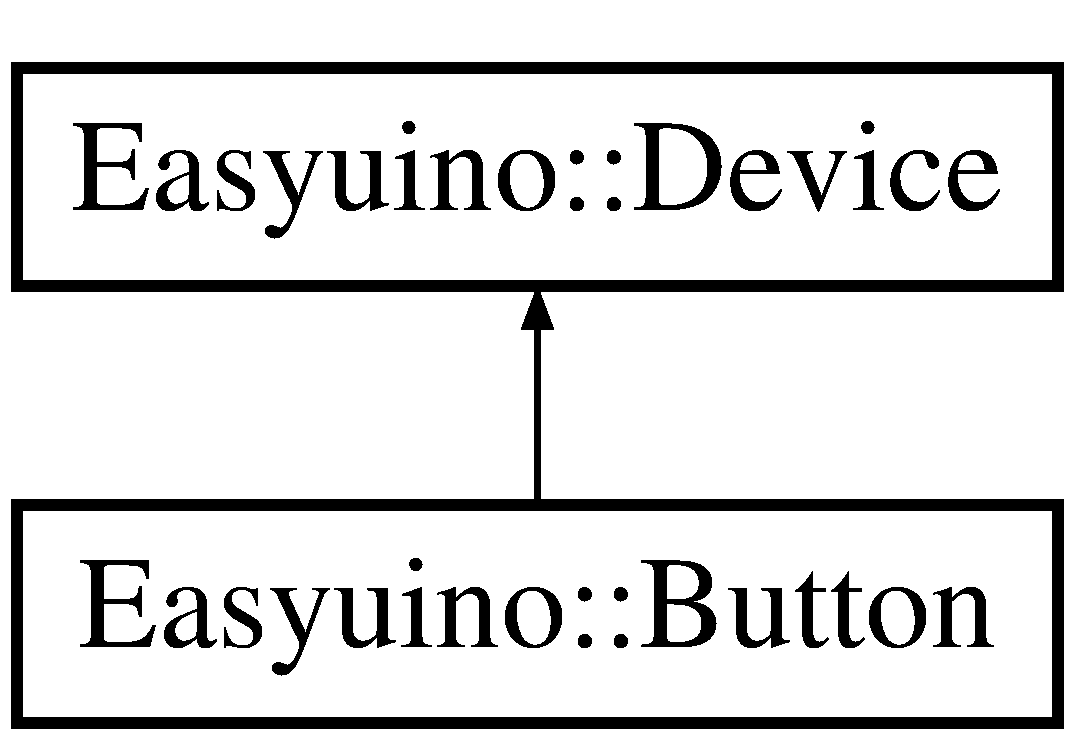
\includegraphics[height=2.000000cm]{class_easyuino_1_1_button}
\end{center}
\end{figure}
\subsection*{Public Member Functions}
\begin{DoxyCompactItemize}
\item 
\hyperlink{class_easyuino_1_1_button_af0b54aae0c20a523d87681bf5f110590}{Button} (IN uint8\+\_\+t button\+Pin)
\begin{DoxyCompactList}\small\item\em Constructor. \end{DoxyCompactList}\item 
\mbox{\Hypertarget{class_easyuino_1_1_button_aecbf28d076ae06ffecf29308aea22d31}\label{class_easyuino_1_1_button_aecbf28d076ae06ffecf29308aea22d31}} 
\hyperlink{class_easyuino_1_1_button_aecbf28d076ae06ffecf29308aea22d31}{$\sim$\+Button} ()
\begin{DoxyCompactList}\small\item\em Destructor. \end{DoxyCompactList}\item 
bool \hyperlink{class_easyuino_1_1_button_a3505f6abb646e92130701d5a1b285c76}{begin} ()
\begin{DoxyCompactList}\small\item\em Used to put the device ready to receive requests. \end{DoxyCompactList}\item 
void \hyperlink{class_easyuino_1_1_button_a0742235d911c24e7b3505f9655176532}{end} ()
\begin{DoxyCompactList}\small\item\em Used to stop the device A\+PI. \end{DoxyCompactList}\item 
bool \hyperlink{class_easyuino_1_1_button_ae0cb534e003379ef6ee49c8589a557ab}{is\+Pressed} ()
\begin{DoxyCompactList}\small\item\em Verifies if the button is pressed. \end{DoxyCompactList}\item 
unsigned long \hyperlink{class_easyuino_1_1_button_a6c2e853db61878dc0050a782dc3eaab9}{get\+Pressed\+Time\+Milliseconds} ()
\begin{DoxyCompactList}\small\item\em Return the the time since it is being pressed. \end{DoxyCompactList}\item 
unsigned int \hyperlink{class_easyuino_1_1_button_a492d3c11c2d437753f51bd25ce305966}{get\+Pressed\+Time\+Seconds} ()
\begin{DoxyCompactList}\small\item\em Return the the time since it is being pressed. \end{DoxyCompactList}\end{DoxyCompactItemize}
\subsection*{Additional Inherited Members}


\subsection{Detailed Description}
\hyperlink{class_easyuino_1_1_button}{Button} A\+PI offers an interface to interact with common buttons. 

\begin{DoxySeeAlso}{See also}
Devices Supported\+: Touch \hyperlink{class_easyuino_1_1_button}{Button} v1.\+0, Push Buttons 

Devices Tested\+: Touch \hyperlink{class_easyuino_1_1_button}{Button} v1.\+0 
\end{DoxySeeAlso}


\subsection{Constructor \& Destructor Documentation}
\mbox{\Hypertarget{class_easyuino_1_1_button_af0b54aae0c20a523d87681bf5f110590}\label{class_easyuino_1_1_button_af0b54aae0c20a523d87681bf5f110590}} 
\index{Easyuino\+::\+Button@{Easyuino\+::\+Button}!Button@{Button}}
\index{Button@{Button}!Easyuino\+::\+Button@{Easyuino\+::\+Button}}
\subsubsection{\texorpdfstring{Button()}{Button()}}
{\footnotesize\ttfamily Easyuino\+::\+Button\+::\+Button (\begin{DoxyParamCaption}\item[{IN uint8\+\_\+t}]{button\+Pin }\end{DoxyParamCaption})}



Constructor. 


\begin{DoxyParams}{Parameters}
{\em button\+Pin} & Arduino pin that is connected to button pin \\
\hline
\end{DoxyParams}


\subsection{Member Function Documentation}
\mbox{\Hypertarget{class_easyuino_1_1_button_a3505f6abb646e92130701d5a1b285c76}\label{class_easyuino_1_1_button_a3505f6abb646e92130701d5a1b285c76}} 
\index{Easyuino\+::\+Button@{Easyuino\+::\+Button}!begin@{begin}}
\index{begin@{begin}!Easyuino\+::\+Button@{Easyuino\+::\+Button}}
\subsubsection{\texorpdfstring{begin()}{begin()}}
{\footnotesize\ttfamily bool Easyuino\+::\+Button\+::begin (\begin{DoxyParamCaption}{ }\end{DoxyParamCaption})\hspace{0.3cm}{\ttfamily [virtual]}}



Used to put the device ready to receive requests. 

Normally this have some default behaviour some devices have other overload method with same name that receives other arguments to device customization. \begin{DoxyReturn}{Returns}
True\+: If the device was initialized. False\+: Otherwise. 
\end{DoxyReturn}


Implements \hyperlink{class_easyuino_1_1_device_a2e7bb2fec849719a9d9432b57cdb72ba}{Easyuino\+::\+Device}.

\mbox{\Hypertarget{class_easyuino_1_1_button_a0742235d911c24e7b3505f9655176532}\label{class_easyuino_1_1_button_a0742235d911c24e7b3505f9655176532}} 
\index{Easyuino\+::\+Button@{Easyuino\+::\+Button}!end@{end}}
\index{end@{end}!Easyuino\+::\+Button@{Easyuino\+::\+Button}}
\subsubsection{\texorpdfstring{end()}{end()}}
{\footnotesize\ttfamily void Easyuino\+::\+Button\+::end (\begin{DoxyParamCaption}{ }\end{DoxyParamCaption})\hspace{0.3cm}{\ttfamily [virtual]}}



Used to stop the device A\+PI. 

After this the the device will not process A\+PI requests. 

Implements \hyperlink{class_easyuino_1_1_device_ab31018ef64adc84aa2ea575b2297548f}{Easyuino\+::\+Device}.

\mbox{\Hypertarget{class_easyuino_1_1_button_a6c2e853db61878dc0050a782dc3eaab9}\label{class_easyuino_1_1_button_a6c2e853db61878dc0050a782dc3eaab9}} 
\index{Easyuino\+::\+Button@{Easyuino\+::\+Button}!get\+Pressed\+Time\+Milliseconds@{get\+Pressed\+Time\+Milliseconds}}
\index{get\+Pressed\+Time\+Milliseconds@{get\+Pressed\+Time\+Milliseconds}!Easyuino\+::\+Button@{Easyuino\+::\+Button}}
\subsubsection{\texorpdfstring{get\+Pressed\+Time\+Milliseconds()}{getPressedTimeMilliseconds()}}
{\footnotesize\ttfamily unsigned long Easyuino\+::\+Button\+::get\+Pressed\+Time\+Milliseconds (\begin{DoxyParamCaption}{ }\end{DoxyParamCaption})}



Return the the time since it is being pressed. 

\begin{DoxyReturn}{Returns}
pressed\+Time Time since the button started being pressed (Milliseconds) OR 0 if button is not being pressed 
\end{DoxyReturn}
\mbox{\Hypertarget{class_easyuino_1_1_button_a492d3c11c2d437753f51bd25ce305966}\label{class_easyuino_1_1_button_a492d3c11c2d437753f51bd25ce305966}} 
\index{Easyuino\+::\+Button@{Easyuino\+::\+Button}!get\+Pressed\+Time\+Seconds@{get\+Pressed\+Time\+Seconds}}
\index{get\+Pressed\+Time\+Seconds@{get\+Pressed\+Time\+Seconds}!Easyuino\+::\+Button@{Easyuino\+::\+Button}}
\subsubsection{\texorpdfstring{get\+Pressed\+Time\+Seconds()}{getPressedTimeSeconds()}}
{\footnotesize\ttfamily unsigned int Easyuino\+::\+Button\+::get\+Pressed\+Time\+Seconds (\begin{DoxyParamCaption}{ }\end{DoxyParamCaption})}



Return the the time since it is being pressed. 

\begin{DoxyReturn}{Returns}
pressed\+Time Time since the button started being pressed (Seconds) OR 0 if button is not being pressed 
\end{DoxyReturn}
\mbox{\Hypertarget{class_easyuino_1_1_button_ae0cb534e003379ef6ee49c8589a557ab}\label{class_easyuino_1_1_button_ae0cb534e003379ef6ee49c8589a557ab}} 
\index{Easyuino\+::\+Button@{Easyuino\+::\+Button}!is\+Pressed@{is\+Pressed}}
\index{is\+Pressed@{is\+Pressed}!Easyuino\+::\+Button@{Easyuino\+::\+Button}}
\subsubsection{\texorpdfstring{is\+Pressed()}{isPressed()}}
{\footnotesize\ttfamily bool Easyuino\+::\+Button\+::is\+Pressed (\begin{DoxyParamCaption}{ }\end{DoxyParamCaption})}



Verifies if the button is pressed. 

\begin{DoxyReturn}{Returns}
is\+Pressed True\+: If button is currently being pressed. False\+: Otherwise. 
\end{DoxyReturn}


The documentation for this class was generated from the following file\+:\begin{DoxyCompactItemize}
\item 
src/Button.\+h\end{DoxyCompactItemize}

\hypertarget{class_easyuino_1_1_device}{}\section{Easyuino\+:\+:Device Class Reference}
\label{class_easyuino_1_1_device}\index{Easyuino\+::\+Device@{Easyuino\+::\+Device}}


General class that provides the common A\+PI behaviour for all the devices/sensors.  




{\ttfamily \#include $<$Device.\+h$>$}

Inheritance diagram for Easyuino\+:\+:Device\+:\begin{figure}[H]
\begin{center}
\leavevmode
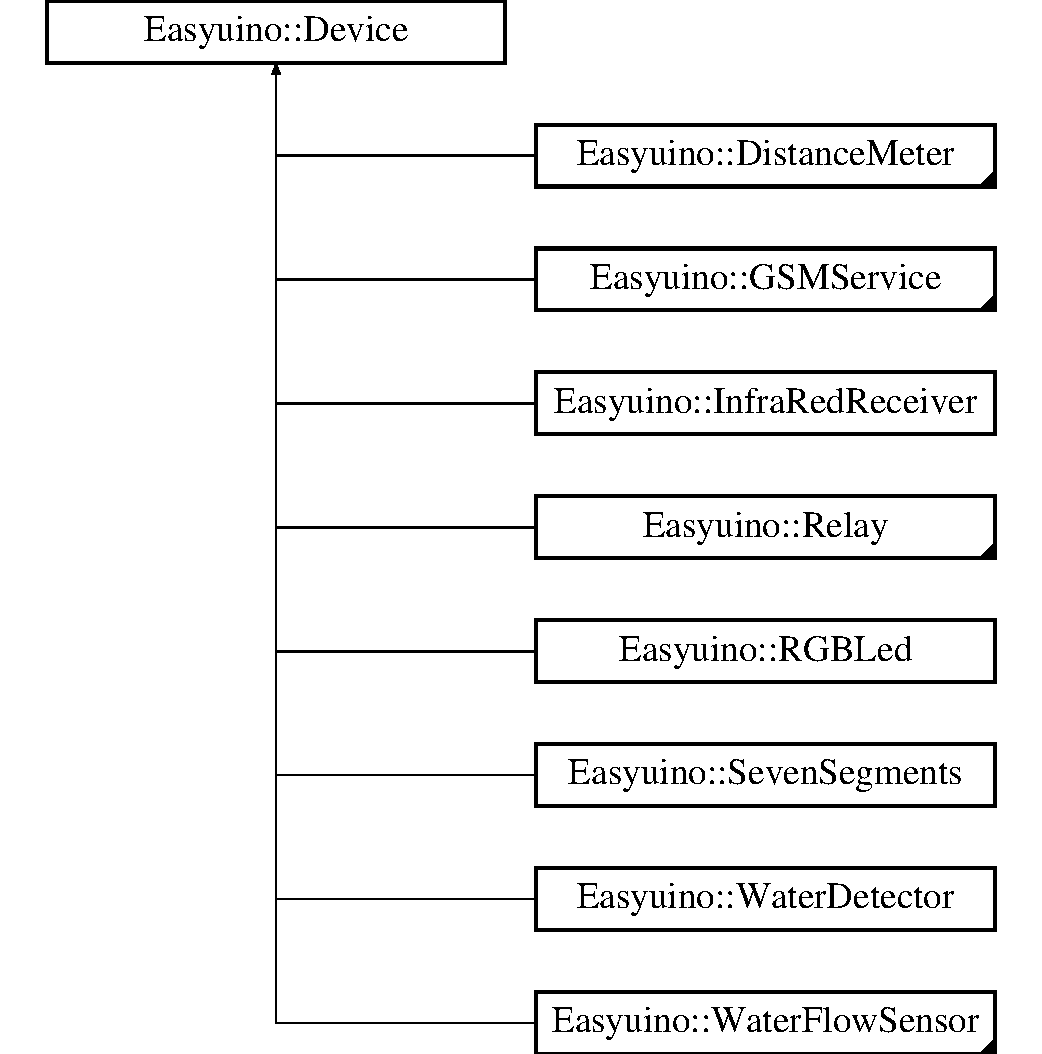
\includegraphics[height=9.000000cm]{class_easyuino_1_1_device}
\end{center}
\end{figure}
\subsection*{Public Member Functions}
\begin{DoxyCompactItemize}
\item 
\mbox{\Hypertarget{class_easyuino_1_1_device_a14b00250154fa77a8c1f766f312c7705}\label{class_easyuino_1_1_device_a14b00250154fa77a8c1f766f312c7705}} 
\hyperlink{class_easyuino_1_1_device_a14b00250154fa77a8c1f766f312c7705}{Device} ()
\begin{DoxyCompactList}\small\item\em Constructor called by every sub-\/classes. \end{DoxyCompactList}\item 
\mbox{\Hypertarget{class_easyuino_1_1_device_a55c8fe2856936c2c770c20da49d5a59d}\label{class_easyuino_1_1_device_a55c8fe2856936c2c770c20da49d5a59d}} 
\hyperlink{class_easyuino_1_1_device_a55c8fe2856936c2c770c20da49d5a59d}{$\sim$\+Device} ()
\begin{DoxyCompactList}\small\item\em Destroy all the resources associated with the device. \end{DoxyCompactList}\item 
virtual bool \hyperlink{class_easyuino_1_1_device_a2e7bb2fec849719a9d9432b57cdb72ba}{begin} ()=0
\begin{DoxyCompactList}\small\item\em Used to put the device ready to receive requests. \end{DoxyCompactList}\item 
virtual void \hyperlink{class_easyuino_1_1_device_ab31018ef64adc84aa2ea575b2297548f}{end} ()=0
\begin{DoxyCompactList}\small\item\em Used to stop the device A\+PI. \end{DoxyCompactList}\item 
bool \hyperlink{class_easyuino_1_1_device_a3761bc02cb81ca0833b535ecaf9a7659}{is\+Initialized} () const
\begin{DoxyCompactList}\small\item\em Verify is the device is initialized and ready to use. \end{DoxyCompactList}\end{DoxyCompactItemize}
\subsection*{Protected Attributes}
\begin{DoxyCompactItemize}
\item 
\mbox{\Hypertarget{class_easyuino_1_1_device_aa0b9574dae06ba9fc2180cba67d63126}\label{class_easyuino_1_1_device_aa0b9574dae06ba9fc2180cba67d63126}} 
bool \hyperlink{class_easyuino_1_1_device_aa0b9574dae06ba9fc2180cba67d63126}{\+\_\+is\+Initialized}
\begin{DoxyCompactList}\small\item\em Used to know if the device A\+PI is initialized and ready to receive requests. \end{DoxyCompactList}\end{DoxyCompactItemize}


\subsection{Detailed Description}
General class that provides the common A\+PI behaviour for all the devices/sensors. 

\subsection{Member Function Documentation}
\mbox{\Hypertarget{class_easyuino_1_1_device_a2e7bb2fec849719a9d9432b57cdb72ba}\label{class_easyuino_1_1_device_a2e7bb2fec849719a9d9432b57cdb72ba}} 
\index{Easyuino\+::\+Device@{Easyuino\+::\+Device}!begin@{begin}}
\index{begin@{begin}!Easyuino\+::\+Device@{Easyuino\+::\+Device}}
\subsubsection{\texorpdfstring{begin()}{begin()}}
{\footnotesize\ttfamily virtual bool Easyuino\+::\+Device\+::begin (\begin{DoxyParamCaption}{ }\end{DoxyParamCaption})\hspace{0.3cm}{\ttfamily [pure virtual]}}



Used to put the device ready to receive requests. 

Normally this have some default behaviour some devices have other overload method with same name that receives other arguments to device customization. \begin{DoxyReturn}{Returns}
True\+: If the device was initialized. False\+: Otherwise. 
\end{DoxyReturn}


Implemented in \hyperlink{class_easyuino_1_1_g_s_m_service_aeafc2dae47e4b13e127eb228a0f7ff6a}{Easyuino\+::\+G\+S\+M\+Service}, \hyperlink{class_easyuino_1_1_r_g_b_led_abdc3512266c7f584609147fccc1ec816}{Easyuino\+::\+R\+G\+B\+Led}, \hyperlink{class_easyuino_1_1_distance_meter_non_block_a46d2093d0fc125e98c3602868c088a77}{Easyuino\+::\+Distance\+Meter\+Non\+Block}, \hyperlink{class_easyuino_1_1_distance_meter_a0374e6f806cd71f0f918c6ea7b7700a0}{Easyuino\+::\+Distance\+Meter}, \hyperlink{class_easyuino_1_1_water_detector_af7a0ec32d6abcb8c1060f493525d5228}{Easyuino\+::\+Water\+Detector}, \hyperlink{class_easyuino_1_1_relay_a920a0fa287cacfd8c6df19d8812d4958}{Easyuino\+::\+Relay}, \hyperlink{class_easyuino_1_1_water_flow_sensor_a55dcab6c527b1e1951a1fff69efdb763}{Easyuino\+::\+Water\+Flow\+Sensor}, \hyperlink{class_easyuino_1_1_water_flow_meter_a400c25b10a7cde45c623805546d071cd}{Easyuino\+::\+Water\+Flow\+Meter}, and \hyperlink{class_easyuino_1_1_seven_segments_ab59d5cbdc22567fb97854f32d899e02d}{Easyuino\+::\+Seven\+Segments}.

\mbox{\Hypertarget{class_easyuino_1_1_device_ab31018ef64adc84aa2ea575b2297548f}\label{class_easyuino_1_1_device_ab31018ef64adc84aa2ea575b2297548f}} 
\index{Easyuino\+::\+Device@{Easyuino\+::\+Device}!end@{end}}
\index{end@{end}!Easyuino\+::\+Device@{Easyuino\+::\+Device}}
\subsubsection{\texorpdfstring{end()}{end()}}
{\footnotesize\ttfamily virtual void Easyuino\+::\+Device\+::end (\begin{DoxyParamCaption}{ }\end{DoxyParamCaption})\hspace{0.3cm}{\ttfamily [pure virtual]}}



Used to stop the device A\+PI. 

After this the the device will not process A\+PI requests. 

Implemented in \hyperlink{class_easyuino_1_1_g_s_m_service_a05bef783773776ec209608aa81d1ff45}{Easyuino\+::\+G\+S\+M\+Service}, \hyperlink{class_easyuino_1_1_r_g_b_led_ad0e9fb0da405c537e876c8a2dc22246e}{Easyuino\+::\+R\+G\+B\+Led}, \hyperlink{class_easyuino_1_1_distance_meter_non_block_a845d4db657ff408205d1cdb3c35982a4}{Easyuino\+::\+Distance\+Meter\+Non\+Block}, \hyperlink{class_easyuino_1_1_distance_meter_a8a818cc922418ae5a078193dbfab1e6b}{Easyuino\+::\+Distance\+Meter}, \hyperlink{class_easyuino_1_1_relay_a2b57237c996a6ffe8e900ae273bce9d4}{Easyuino\+::\+Relay}, \hyperlink{class_easyuino_1_1_water_detector_a9c1473536f47b2a7d8e1f8fb1bf5f3fd}{Easyuino\+::\+Water\+Detector}, \hyperlink{class_easyuino_1_1_water_flow_sensor_a7f31ac7735b049394d34cfbc37f17359}{Easyuino\+::\+Water\+Flow\+Sensor}, \hyperlink{class_easyuino_1_1_water_flow_meter_a47024d4da9568e42743a875c08c33121}{Easyuino\+::\+Water\+Flow\+Meter}, and \hyperlink{class_easyuino_1_1_seven_segments_afea49385382a7b9c597b4fe42a003fee}{Easyuino\+::\+Seven\+Segments}.

\mbox{\Hypertarget{class_easyuino_1_1_device_a3761bc02cb81ca0833b535ecaf9a7659}\label{class_easyuino_1_1_device_a3761bc02cb81ca0833b535ecaf9a7659}} 
\index{Easyuino\+::\+Device@{Easyuino\+::\+Device}!is\+Initialized@{is\+Initialized}}
\index{is\+Initialized@{is\+Initialized}!Easyuino\+::\+Device@{Easyuino\+::\+Device}}
\subsubsection{\texorpdfstring{is\+Initialized()}{isInitialized()}}
{\footnotesize\ttfamily bool Easyuino\+::\+Device\+::is\+Initialized (\begin{DoxyParamCaption}{ }\end{DoxyParamCaption}) const}



Verify is the device is initialized and ready to use. 

\begin{DoxyReturn}{Returns}
True\+: If device is initialized. False\+: Otherwise. 
\end{DoxyReturn}


The documentation for this class was generated from the following file\+:\begin{DoxyCompactItemize}
\item 
src/Device.\+h\end{DoxyCompactItemize}

\hypertarget{class_easyuino_1_1_distance_meter}{}\section{Easyuino\+:\+:Distance\+Meter Class Reference}
\label{class_easyuino_1_1_distance_meter}\index{Easyuino\+::\+Distance\+Meter@{Easyuino\+::\+Distance\+Meter}}


Used to represent the at least supported Ultrasonic Module models enum Ultrasonic\+Module \+: uint8\+\_\+t \{ H\+C\+\_\+\+S\+R03, H\+C\+\_\+\+S\+R04, H\+C\+\_\+\+S\+R05 \};.  




{\ttfamily \#include $<$Distance\+Meter.\+h$>$}

Inheritance diagram for Easyuino\+:\+:Distance\+Meter\+:\begin{figure}[H]
\begin{center}
\leavevmode
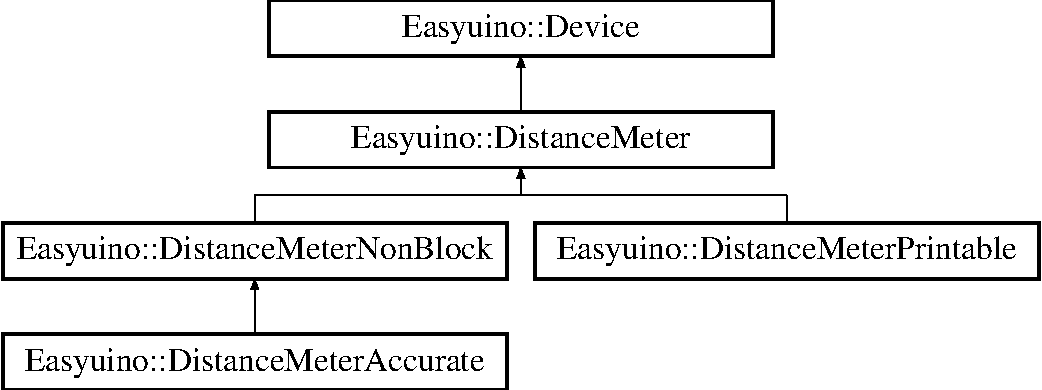
\includegraphics[height=4.000000cm]{class_easyuino_1_1_distance_meter}
\end{center}
\end{figure}
\subsection*{Public Member Functions}
\begin{DoxyCompactItemize}
\item 
\hyperlink{class_easyuino_1_1_distance_meter_aad61ebf8398ba5cf6a80e5defc29bfcc}{Distance\+Meter} (IN uint8\+\_\+t trigger\+Pin, IN uint8\+\_\+t echo\+Pin)
\begin{DoxyCompactList}\small\item\em Constructor. \end{DoxyCompactList}\item 
\hyperlink{class_easyuino_1_1_distance_meter_aa5551cc3c42fe77f0972a41acf896cf9}{Distance\+Meter} (IN uint8\+\_\+t trigger\+Echo\+Pin)
\begin{DoxyCompactList}\small\item\em Contructor used with Ultrasonic Modules that have only one pin for trigger and echo. \end{DoxyCompactList}\item 
\mbox{\Hypertarget{class_easyuino_1_1_distance_meter_aacd298add519e79000e08a7bb1995d0f}\label{class_easyuino_1_1_distance_meter_aacd298add519e79000e08a7bb1995d0f}} 
\hyperlink{class_easyuino_1_1_distance_meter_aacd298add519e79000e08a7bb1995d0f}{$\sim$\+Distance\+Meter} ()
\begin{DoxyCompactList}\small\item\em Destructor. \end{DoxyCompactList}\item 
bool \hyperlink{class_easyuino_1_1_distance_meter_a0374e6f806cd71f0f918c6ea7b7700a0}{begin} ()
\begin{DoxyCompactList}\small\item\em Used to put the device ready to receive requests. \end{DoxyCompactList}\item 
void \hyperlink{class_easyuino_1_1_distance_meter_a8a818cc922418ae5a078193dbfab1e6b}{end} ()
\begin{DoxyCompactList}\small\item\em Used to stop the device A\+PI. \end{DoxyCompactList}\item 
virtual float \hyperlink{class_easyuino_1_1_distance_meter_a637cdd0d3e4f3bcf094704ae91e0c7c3}{get\+Distance\+Centimeters} ()
\begin{DoxyCompactList}\small\item\em Gets the last value that the A\+PI measured using the Ultrasonic Module. \end{DoxyCompactList}\item 
float \hyperlink{class_easyuino_1_1_distance_meter_a4e3c650c54382d9af6bca51dcac4e7a3}{get\+Distance\+Inches} ()
\begin{DoxyCompactList}\small\item\em Gets the last value that the A\+PI measured using the US. \end{DoxyCompactList}\item 
virtual void \hyperlink{class_easyuino_1_1_distance_meter_a739197578f06b58faedefd0526d49499}{update\+Distance} ()
\begin{DoxyCompactList}\small\item\em Updates the distance of the Ultrasonic Module to the objects in a blocking way. \end{DoxyCompactList}\end{DoxyCompactItemize}
\subsection*{Protected Member Functions}
\begin{DoxyCompactItemize}
\item 
float \hyperlink{class_easyuino_1_1_distance_meter_a4e02477669d61a3a7afb7deb9c53cf17}{execute\+Update\+Distance\+Block} (IN float sound\+Speed)
\begin{DoxyCompactList}\small\item\em Execute a block distance measurement and calculates the distance based on the sound speed. \end{DoxyCompactList}\end{DoxyCompactItemize}
\subsection*{Protected Attributes}
\begin{DoxyCompactItemize}
\item 
\mbox{\Hypertarget{class_easyuino_1_1_distance_meter_a39f2305fe998cd3212eef389dfe036fe}\label{class_easyuino_1_1_distance_meter_a39f2305fe998cd3212eef389dfe036fe}} 
uint8\+\_\+t \hyperlink{class_easyuino_1_1_distance_meter_a39f2305fe998cd3212eef389dfe036fe}{\+\_\+trigger\+Pin}
\begin{DoxyCompactList}\small\item\em Arduino pin used to trigger the echo wave emission. \end{DoxyCompactList}\item 
\mbox{\Hypertarget{class_easyuino_1_1_distance_meter_a6f4a18c48dc147102f1fae8cb12e24a2}\label{class_easyuino_1_1_distance_meter_a6f4a18c48dc147102f1fae8cb12e24a2}} 
uint8\+\_\+t \hyperlink{class_easyuino_1_1_distance_meter_a6f4a18c48dc147102f1fae8cb12e24a2}{\+\_\+echo\+Pin}
\begin{DoxyCompactList}\small\item\em Arduino pin that is set to L\+OW by when reflected echo wave arrives. \end{DoxyCompactList}\item 
\mbox{\Hypertarget{class_easyuino_1_1_distance_meter_ae2b9e4d3e8704c8f1a73639afd53614d}\label{class_easyuino_1_1_distance_meter_ae2b9e4d3e8704c8f1a73639afd53614d}} 
volatile bool \hyperlink{class_easyuino_1_1_distance_meter_ae2b9e4d3e8704c8f1a73639afd53614d}{\+\_\+is\+Echoing}
\begin{DoxyCompactList}\small\item\em Used to know if it is in a middle of a measurement. \end{DoxyCompactList}\item 
volatile float \hyperlink{class_easyuino_1_1_distance_meter_ae10df1a21d2acfec3aa3eef57ea3a632}{\+\_\+distance}
\begin{DoxyCompactList}\small\item\em It contains a cached value of the last distance measured. \end{DoxyCompactList}\end{DoxyCompactItemize}


\subsection{Detailed Description}
Used to represent the at least supported Ultrasonic Module models enum Ultrasonic\+Module \+: uint8\+\_\+t \{ H\+C\+\_\+\+S\+R03, H\+C\+\_\+\+S\+R04, H\+C\+\_\+\+S\+R05 \};. 

\hyperlink{class_easyuino_1_1_distance_meter}{Distance\+Meter} offers a simple A\+PI to interact with an Ultrasonic Module to measure distances to objects. \begin{DoxySeeAlso}{See also}
Devices Supported\+: H\+C-\/\+S\+R03, H\+C-\/\+S\+R04, H\+C-\/\+S\+R05 

Devices Tested\+: H\+C-\/\+S\+R04 
\end{DoxySeeAlso}


\subsection{Constructor \& Destructor Documentation}
\mbox{\Hypertarget{class_easyuino_1_1_distance_meter_aad61ebf8398ba5cf6a80e5defc29bfcc}\label{class_easyuino_1_1_distance_meter_aad61ebf8398ba5cf6a80e5defc29bfcc}} 
\index{Easyuino\+::\+Distance\+Meter@{Easyuino\+::\+Distance\+Meter}!Distance\+Meter@{Distance\+Meter}}
\index{Distance\+Meter@{Distance\+Meter}!Easyuino\+::\+Distance\+Meter@{Easyuino\+::\+Distance\+Meter}}
\subsubsection{\texorpdfstring{Distance\+Meter()}{DistanceMeter()}\hspace{0.1cm}{\footnotesize\ttfamily [1/2]}}
{\footnotesize\ttfamily Easyuino\+::\+Distance\+Meter\+::\+Distance\+Meter (\begin{DoxyParamCaption}\item[{IN uint8\+\_\+t}]{trigger\+Pin,  }\item[{IN uint8\+\_\+t}]{echo\+Pin }\end{DoxyParamCaption})}



Constructor. 


\begin{DoxyParams}{Parameters}
{\em trigger\+Pin} & Arduino pin connected to the trigger pin of the Ultrasonic Module \\
\hline
{\em echo\+Pin} & Arduino pin connected to the echo pin of the Ultrasonic Module \\
\hline
\end{DoxyParams}
\mbox{\Hypertarget{class_easyuino_1_1_distance_meter_aa5551cc3c42fe77f0972a41acf896cf9}\label{class_easyuino_1_1_distance_meter_aa5551cc3c42fe77f0972a41acf896cf9}} 
\index{Easyuino\+::\+Distance\+Meter@{Easyuino\+::\+Distance\+Meter}!Distance\+Meter@{Distance\+Meter}}
\index{Distance\+Meter@{Distance\+Meter}!Easyuino\+::\+Distance\+Meter@{Easyuino\+::\+Distance\+Meter}}
\subsubsection{\texorpdfstring{Distance\+Meter()}{DistanceMeter()}\hspace{0.1cm}{\footnotesize\ttfamily [2/2]}}
{\footnotesize\ttfamily Easyuino\+::\+Distance\+Meter\+::\+Distance\+Meter (\begin{DoxyParamCaption}\item[{IN uint8\+\_\+t}]{trigger\+Echo\+Pin }\end{DoxyParamCaption})}



Contructor used with Ultrasonic Modules that have only one pin for trigger and echo. 


\begin{DoxyParams}{Parameters}
{\em trigger\+Echo\+Pin} & Arduino pin connected to the trigger\&echo pin of the Ultrasonic Module \\
\hline
\end{DoxyParams}


\subsection{Member Function Documentation}
\mbox{\Hypertarget{class_easyuino_1_1_distance_meter_a0374e6f806cd71f0f918c6ea7b7700a0}\label{class_easyuino_1_1_distance_meter_a0374e6f806cd71f0f918c6ea7b7700a0}} 
\index{Easyuino\+::\+Distance\+Meter@{Easyuino\+::\+Distance\+Meter}!begin@{begin}}
\index{begin@{begin}!Easyuino\+::\+Distance\+Meter@{Easyuino\+::\+Distance\+Meter}}
\subsubsection{\texorpdfstring{begin()}{begin()}}
{\footnotesize\ttfamily bool Easyuino\+::\+Distance\+Meter\+::begin (\begin{DoxyParamCaption}{ }\end{DoxyParamCaption})\hspace{0.3cm}{\ttfamily [virtual]}}



Used to put the device ready to receive requests. 

Normally this have some default behaviour some devices have other overload method with same name that receives other arguments to device customization. \begin{DoxyReturn}{Returns}
True\+: If the device was initialized. False\+: Otherwise. 
\end{DoxyReturn}


Implements \hyperlink{class_easyuino_1_1_device_a2e7bb2fec849719a9d9432b57cdb72ba}{Easyuino\+::\+Device}.



Reimplemented in \hyperlink{class_easyuino_1_1_distance_meter_non_block_a46d2093d0fc125e98c3602868c088a77}{Easyuino\+::\+Distance\+Meter\+Non\+Block}.

\mbox{\Hypertarget{class_easyuino_1_1_distance_meter_a8a818cc922418ae5a078193dbfab1e6b}\label{class_easyuino_1_1_distance_meter_a8a818cc922418ae5a078193dbfab1e6b}} 
\index{Easyuino\+::\+Distance\+Meter@{Easyuino\+::\+Distance\+Meter}!end@{end}}
\index{end@{end}!Easyuino\+::\+Distance\+Meter@{Easyuino\+::\+Distance\+Meter}}
\subsubsection{\texorpdfstring{end()}{end()}}
{\footnotesize\ttfamily void Easyuino\+::\+Distance\+Meter\+::end (\begin{DoxyParamCaption}{ }\end{DoxyParamCaption})\hspace{0.3cm}{\ttfamily [virtual]}}



Used to stop the device A\+PI. 

After this the the device will not process A\+PI requests. 

Implements \hyperlink{class_easyuino_1_1_device_ab31018ef64adc84aa2ea575b2297548f}{Easyuino\+::\+Device}.



Reimplemented in \hyperlink{class_easyuino_1_1_distance_meter_non_block_a845d4db657ff408205d1cdb3c35982a4}{Easyuino\+::\+Distance\+Meter\+Non\+Block}.

\mbox{\Hypertarget{class_easyuino_1_1_distance_meter_a4e02477669d61a3a7afb7deb9c53cf17}\label{class_easyuino_1_1_distance_meter_a4e02477669d61a3a7afb7deb9c53cf17}} 
\index{Easyuino\+::\+Distance\+Meter@{Easyuino\+::\+Distance\+Meter}!execute\+Update\+Distance\+Block@{execute\+Update\+Distance\+Block}}
\index{execute\+Update\+Distance\+Block@{execute\+Update\+Distance\+Block}!Easyuino\+::\+Distance\+Meter@{Easyuino\+::\+Distance\+Meter}}
\subsubsection{\texorpdfstring{execute\+Update\+Distance\+Block()}{executeUpdateDistanceBlock()}}
{\footnotesize\ttfamily float Easyuino\+::\+Distance\+Meter\+::execute\+Update\+Distance\+Block (\begin{DoxyParamCaption}\item[{IN float}]{sound\+Speed }\end{DoxyParamCaption})\hspace{0.3cm}{\ttfamily [protected]}}



Execute a block distance measurement and calculates the distance based on the sound speed. 


\begin{DoxyParams}{Parameters}
{\em sound\+Speed} & (Cm/\+Sec) Sound speed to introduce in the calculation \\
\hline
\end{DoxyParams}
\begin{DoxyReturn}{Returns}
distance (Centimeters) The new distance measured 
\end{DoxyReturn}
\mbox{\Hypertarget{class_easyuino_1_1_distance_meter_a637cdd0d3e4f3bcf094704ae91e0c7c3}\label{class_easyuino_1_1_distance_meter_a637cdd0d3e4f3bcf094704ae91e0c7c3}} 
\index{Easyuino\+::\+Distance\+Meter@{Easyuino\+::\+Distance\+Meter}!get\+Distance\+Centimeters@{get\+Distance\+Centimeters}}
\index{get\+Distance\+Centimeters@{get\+Distance\+Centimeters}!Easyuino\+::\+Distance\+Meter@{Easyuino\+::\+Distance\+Meter}}
\subsubsection{\texorpdfstring{get\+Distance\+Centimeters()}{getDistanceCentimeters()}}
{\footnotesize\ttfamily virtual float Easyuino\+::\+Distance\+Meter\+::get\+Distance\+Centimeters (\begin{DoxyParamCaption}{ }\end{DoxyParamCaption})\hspace{0.3cm}{\ttfamily [virtual]}}



Gets the last value that the A\+PI measured using the Ultrasonic Module. 

\begin{DoxyReturn}{Returns}
distance (Centimeters) The most recent measurement the A\+PI have done 
\end{DoxyReturn}


Reimplemented in \hyperlink{class_easyuino_1_1_distance_meter_non_block_a00419fc2c2ff7c587735063971aa7464}{Easyuino\+::\+Distance\+Meter\+Non\+Block}, and \hyperlink{class_easyuino_1_1_distance_meter_accurate_a4de44a347db0bebbf5d74f12397cd4d9}{Easyuino\+::\+Distance\+Meter\+Accurate}.

\mbox{\Hypertarget{class_easyuino_1_1_distance_meter_a4e3c650c54382d9af6bca51dcac4e7a3}\label{class_easyuino_1_1_distance_meter_a4e3c650c54382d9af6bca51dcac4e7a3}} 
\index{Easyuino\+::\+Distance\+Meter@{Easyuino\+::\+Distance\+Meter}!get\+Distance\+Inches@{get\+Distance\+Inches}}
\index{get\+Distance\+Inches@{get\+Distance\+Inches}!Easyuino\+::\+Distance\+Meter@{Easyuino\+::\+Distance\+Meter}}
\subsubsection{\texorpdfstring{get\+Distance\+Inches()}{getDistanceInches()}}
{\footnotesize\ttfamily float Easyuino\+::\+Distance\+Meter\+::get\+Distance\+Inches (\begin{DoxyParamCaption}{ }\end{DoxyParamCaption})}



Gets the last value that the A\+PI measured using the US. 

\begin{DoxyReturn}{Returns}
distance (Inches) The most recent measurement the A\+PI have done 
\end{DoxyReturn}
\mbox{\Hypertarget{class_easyuino_1_1_distance_meter_a739197578f06b58faedefd0526d49499}\label{class_easyuino_1_1_distance_meter_a739197578f06b58faedefd0526d49499}} 
\index{Easyuino\+::\+Distance\+Meter@{Easyuino\+::\+Distance\+Meter}!update\+Distance@{update\+Distance}}
\index{update\+Distance@{update\+Distance}!Easyuino\+::\+Distance\+Meter@{Easyuino\+::\+Distance\+Meter}}
\subsubsection{\texorpdfstring{update\+Distance()}{updateDistance()}}
{\footnotesize\ttfamily virtual void Easyuino\+::\+Distance\+Meter\+::update\+Distance (\begin{DoxyParamCaption}{ }\end{DoxyParamCaption})\hspace{0.3cm}{\ttfamily [virtual]}}



Updates the distance of the Ultrasonic Module to the objects in a blocking way. 

The new distance value is available using \hyperlink{class_easyuino_1_1_distance_meter_a637cdd0d3e4f3bcf094704ae91e0c7c3}{get\+Distance\+Centimeters()} or \hyperlink{class_easyuino_1_1_distance_meter_a4e3c650c54382d9af6bca51dcac4e7a3}{get\+Distance\+Inches()} method after calling this method. \begin{DoxyWarning}{Warning}
This method blocks while the measurement is on going, so the arduino waits for the measure to be concluded, if you want a non block update distance method look for \hyperlink{class_easyuino_1_1_distance_meter_non_block}{Distance\+Meter\+Non\+Block} A\+PI 
\end{DoxyWarning}


Reimplemented in \hyperlink{class_easyuino_1_1_distance_meter_non_block_a4ea37c6c0562a76cd03636db329743f9}{Easyuino\+::\+Distance\+Meter\+Non\+Block}.



\subsection{Member Data Documentation}
\mbox{\Hypertarget{class_easyuino_1_1_distance_meter_ae10df1a21d2acfec3aa3eef57ea3a632}\label{class_easyuino_1_1_distance_meter_ae10df1a21d2acfec3aa3eef57ea3a632}} 
\index{Easyuino\+::\+Distance\+Meter@{Easyuino\+::\+Distance\+Meter}!\+\_\+distance@{\+\_\+distance}}
\index{\+\_\+distance@{\+\_\+distance}!Easyuino\+::\+Distance\+Meter@{Easyuino\+::\+Distance\+Meter}}
\subsubsection{\texorpdfstring{\+\_\+distance}{\_distance}}
{\footnotesize\ttfamily volatile float Easyuino\+::\+Distance\+Meter\+::\+\_\+distance\hspace{0.3cm}{\ttfamily [protected]}}



It contains a cached value of the last distance measured. 

Avoid calculate all the time. 

The documentation for this class was generated from the following file\+:\begin{DoxyCompactItemize}
\item 
src/Distance\+Meter.\+h\end{DoxyCompactItemize}

\hypertarget{class_easyuino_1_1_distance_meter_accurate}{}\section{Easyuino\+:\+:Distance\+Meter\+Accurate Class Reference}
\label{class_easyuino_1_1_distance_meter_accurate}\index{Easyuino\+::\+Distance\+Meter\+Accurate@{Easyuino\+::\+Distance\+Meter\+Accurate}}
Inheritance diagram for Easyuino\+:\+:Distance\+Meter\+Accurate\+:\begin{figure}[H]
\begin{center}
\leavevmode
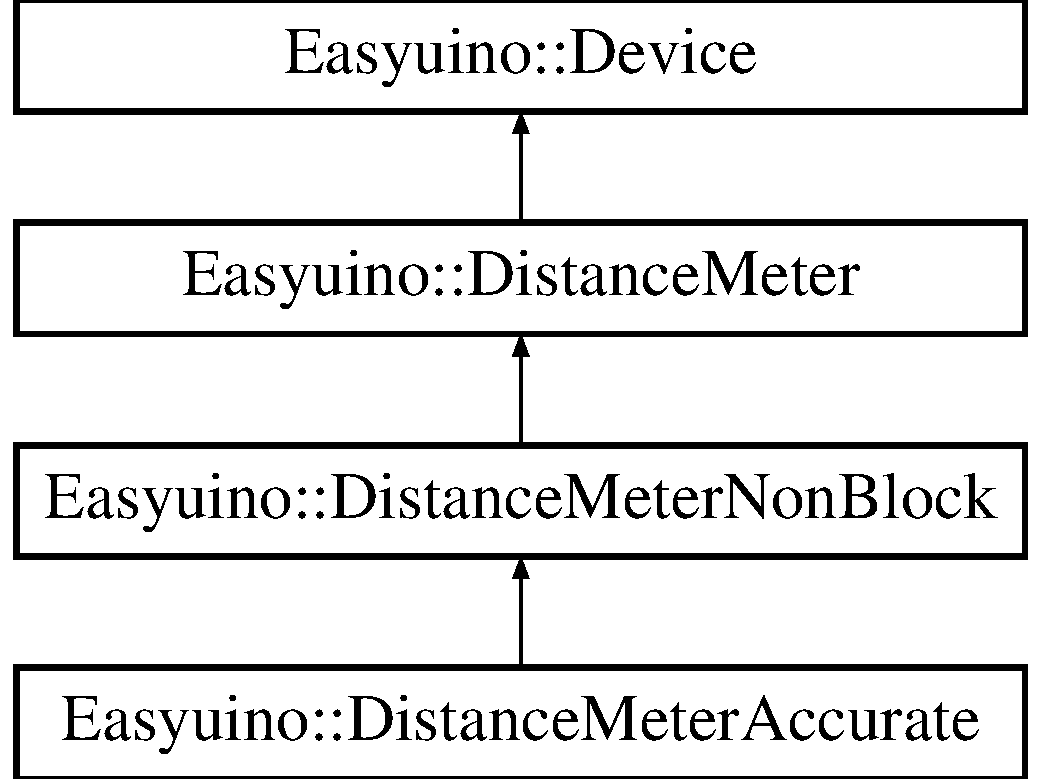
\includegraphics[height=4.000000cm]{class_easyuino_1_1_distance_meter_accurate}
\end{center}
\end{figure}
\subsection*{Public Member Functions}
\begin{DoxyCompactItemize}
\item 
\mbox{\Hypertarget{class_easyuino_1_1_distance_meter_accurate_a57f810d7e6653028bc23139e703985d7}\label{class_easyuino_1_1_distance_meter_accurate_a57f810d7e6653028bc23139e703985d7}} 
{\bfseries Distance\+Meter\+Accurate} (IN uint8\+\_\+t trigger\+Pin, IN uint8\+\_\+t echo\+Pin)
\item 
\mbox{\Hypertarget{class_easyuino_1_1_distance_meter_accurate_a6e58a043f9d28dd6c7e4c5b819607341}\label{class_easyuino_1_1_distance_meter_accurate_a6e58a043f9d28dd6c7e4c5b819607341}} 
{\bfseries Distance\+Meter\+Accurate} (IN uint8\+\_\+t trigger\+Echo\+Pin)
\item 
\mbox{\Hypertarget{class_easyuino_1_1_distance_meter_accurate_a4de44a347db0bebbf5d74f12397cd4d9}\label{class_easyuino_1_1_distance_meter_accurate_a4de44a347db0bebbf5d74f12397cd4d9}} 
float {\bfseries get\+Distance\+Centimeters} ()
\item 
void \hyperlink{class_easyuino_1_1_distance_meter_accurate_af7c43ebaa1ae75db2f806dc7039c8a82}{update\+Distance} (IN float air\+Temperature=D\+E\+F\+A\+U\+L\+T\+\_\+\+A\+I\+R\+\_\+\+T\+E\+M\+P\+E\+R\+A\+T\+U\+R\+E\+\_\+\+C\+E\+L\+S\+I\+US, IN Temperature\+Scale temperature\+Scale=C\+E\+L\+S\+I\+US)
\begin{DoxyCompactList}\small\item\em Updates the distance of the US to the objects in a blocking way. \end{DoxyCompactList}\item 
\mbox{\Hypertarget{class_easyuino_1_1_distance_meter_accurate_ac428b0dfd816862fab277b2da1f0c164}\label{class_easyuino_1_1_distance_meter_accurate_ac428b0dfd816862fab277b2da1f0c164}} 
void {\bfseries update\+Distance\+Non\+Block} (IN float air\+Temperature=D\+E\+F\+A\+U\+L\+T\+\_\+\+A\+I\+R\+\_\+\+T\+E\+M\+P\+E\+R\+A\+T\+U\+R\+E\+\_\+\+C\+E\+L\+S\+I\+US, IN Temperature\+Scale temperature\+Scale=C\+E\+L\+S\+I\+US)
\end{DoxyCompactItemize}
\subsection*{Additional Inherited Members}


\subsection{Member Function Documentation}
\mbox{\Hypertarget{class_easyuino_1_1_distance_meter_accurate_af7c43ebaa1ae75db2f806dc7039c8a82}\label{class_easyuino_1_1_distance_meter_accurate_af7c43ebaa1ae75db2f806dc7039c8a82}} 
\index{Easyuino\+::\+Distance\+Meter\+Accurate@{Easyuino\+::\+Distance\+Meter\+Accurate}!update\+Distance@{update\+Distance}}
\index{update\+Distance@{update\+Distance}!Easyuino\+::\+Distance\+Meter\+Accurate@{Easyuino\+::\+Distance\+Meter\+Accurate}}
\subsubsection{\texorpdfstring{update\+Distance()}{updateDistance()}}
{\footnotesize\ttfamily void Easyuino\+::\+Distance\+Meter\+Accurate\+::update\+Distance (\begin{DoxyParamCaption}\item[{IN float}]{air\+Temperature = {\ttfamily DEFAULT\+\_\+AIR\+\_\+TEMPERATURE\+\_\+CELSIUS},  }\item[{IN Temperature\+Scale}]{temperature\+Scale = {\ttfamily CELSIUS} }\end{DoxyParamCaption})}



Updates the distance of the US to the objects in a blocking way. 

Basically if update\+Distance\+Non\+Block was not called in the last 3 secs at least the method will block on call and when it finishes the distance value can be grabbed by get\+Distance method. 
\begin{DoxyParams}{Parameters}
{\em air\+Temperature} & -\/ Air temperatures to be used when calculating the distance (good if it is the current temperature) \\
\hline
{\em temperature\+Scale} & -\/ The temperature scale that is being provided (C\+E\+L\+S\+I\+US, K\+E\+L\+V\+IN or F\+A\+H\+R\+E\+N\+H\+E\+IT) \\
\hline
\end{DoxyParams}


The documentation for this class was generated from the following files\+:\begin{DoxyCompactItemize}
\item 
src/Distance\+Meter\+Accurate.\+h\item 
src/main/\+Ultrasonic/Distance\+Meter\+Accurate.\+cpp\end{DoxyCompactItemize}

\hypertarget{class_easyuino_1_1_distance_meter_non_block}{}\section{Easyuino\+:\+:Distance\+Meter\+Non\+Block Class Reference}
\label{class_easyuino_1_1_distance_meter_non_block}\index{Easyuino\+::\+Distance\+Meter\+Non\+Block@{Easyuino\+::\+Distance\+Meter\+Non\+Block}}


\hyperlink{class_easyuino_1_1_distance_meter_non_block}{Distance\+Meter\+Non\+Block} offers an A\+PI to interact with an Ultrasonic Module to measure distance in a non-\/block way.  




{\ttfamily \#include $<$Distance\+Meter\+Non\+Block.\+h$>$}

Inheritance diagram for Easyuino\+:\+:Distance\+Meter\+Non\+Block\+:\begin{figure}[H]
\begin{center}
\leavevmode
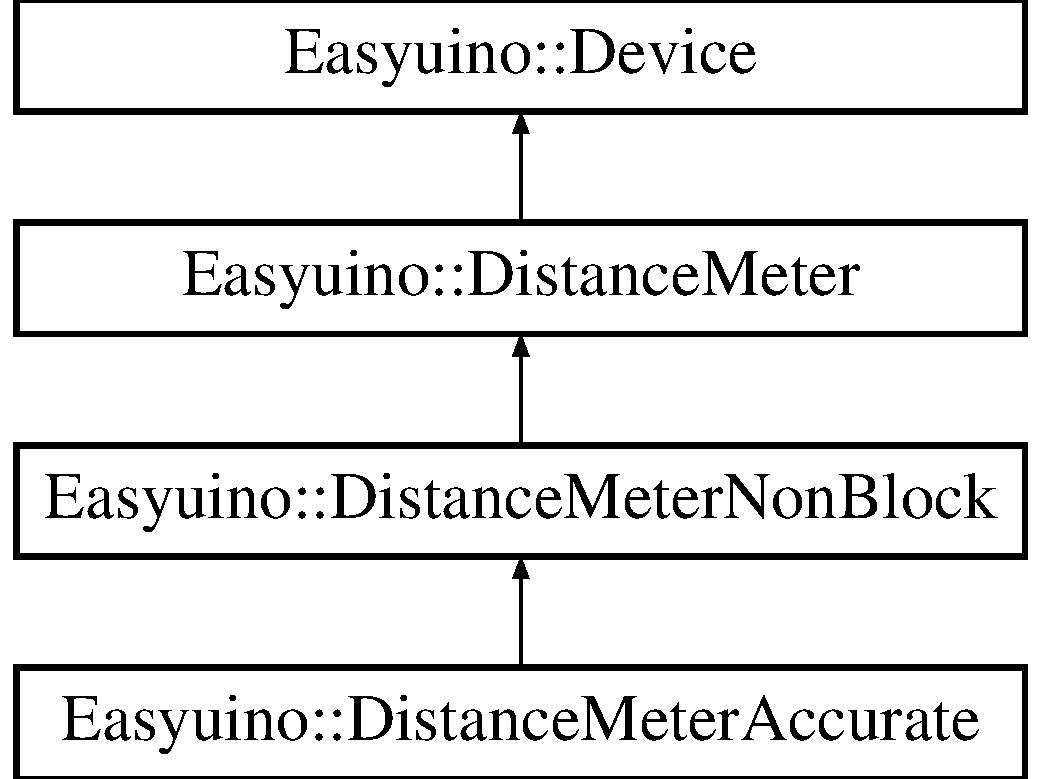
\includegraphics[height=4.000000cm]{class_easyuino_1_1_distance_meter_non_block}
\end{center}
\end{figure}
\subsection*{Public Member Functions}
\begin{DoxyCompactItemize}
\item 
\hyperlink{class_easyuino_1_1_distance_meter_non_block_ad7e7b63fc4655957eb00f24d82512d2a}{Distance\+Meter\+Non\+Block} (IN uint8\+\_\+t trigger\+Pin, IN uint8\+\_\+t echo\+Pin)
\begin{DoxyCompactList}\small\item\em Constructor. \end{DoxyCompactList}\item 
\hyperlink{class_easyuino_1_1_distance_meter_non_block_af77c0f4649ea521a5b75c457b6762db2}{Distance\+Meter\+Non\+Block} (IN uint8\+\_\+t trigger\+Echo\+Pin)
\begin{DoxyCompactList}\small\item\em Contructor used with Ultrasonic Modules that have only one pin for trigger and echo. \end{DoxyCompactList}\item 
\mbox{\Hypertarget{class_easyuino_1_1_distance_meter_non_block_aabd746582e5f4dbca115e6459249e002}\label{class_easyuino_1_1_distance_meter_non_block_aabd746582e5f4dbca115e6459249e002}} 
\hyperlink{class_easyuino_1_1_distance_meter_non_block_aabd746582e5f4dbca115e6459249e002}{$\sim$\+Distance\+Meter\+Non\+Block} ()
\begin{DoxyCompactList}\small\item\em Destructor. \end{DoxyCompactList}\item 
bool \hyperlink{class_easyuino_1_1_distance_meter_non_block_a46d2093d0fc125e98c3602868c088a77}{begin} ()
\begin{DoxyCompactList}\small\item\em Used to put the device ready to receive requests. \end{DoxyCompactList}\item 
void \hyperlink{class_easyuino_1_1_distance_meter_non_block_a845d4db657ff408205d1cdb3c35982a4}{end} ()
\begin{DoxyCompactList}\small\item\em Used to stop the device A\+PI. \end{DoxyCompactList}\item 
float \hyperlink{class_easyuino_1_1_distance_meter_non_block_a00419fc2c2ff7c587735063971aa7464}{get\+Distance\+Centimeters} ()
\begin{DoxyCompactList}\small\item\em Gets the last value that the A\+PI measured using the Ultrasonic Module. \end{DoxyCompactList}\item 
void \hyperlink{class_easyuino_1_1_distance_meter_non_block_a4ea37c6c0562a76cd03636db329743f9}{update\+Distance} ()
\begin{DoxyCompactList}\small\item\em Updates the distance of the Ultrasonic Module to the objects in a blocking way. \end{DoxyCompactList}\item 
virtual void \hyperlink{class_easyuino_1_1_distance_meter_non_block_ac7163baab744f1393bab3841de0170d4}{update\+Distance\+Non\+Block} ()
\begin{DoxyCompactList}\small\item\em Updates the distance of the Ultrasonic Module to the objects in a non-\/blocking way. \end{DoxyCompactList}\end{DoxyCompactItemize}
\subsection*{Protected Member Functions}
\begin{DoxyCompactItemize}
\item 
\mbox{\Hypertarget{class_easyuino_1_1_distance_meter_non_block_a5410be2725e26c878ebf9bcdf2b79a05}\label{class_easyuino_1_1_distance_meter_non_block_a5410be2725e26c878ebf9bcdf2b79a05}} 
void \hyperlink{class_easyuino_1_1_distance_meter_non_block_a5410be2725e26c878ebf9bcdf2b79a05}{execute\+Update\+Distance\+Non\+Block} ()
\begin{DoxyCompactList}\small\item\em Execute a non-\/block distance measurement. \end{DoxyCompactList}\item 
bool \hyperlink{class_easyuino_1_1_distance_meter_non_block_a88f2b7e249345b93a8258ae5c7b75a49}{is\+Update\+Distance\+Non\+Block\+Timeout} ()
\begin{DoxyCompactList}\small\item\em Verify if there is a non-\/block measuremenet on going that has already timeouted. \end{DoxyCompactList}\item 
float \hyperlink{class_easyuino_1_1_distance_meter_non_block_aa51eb173540f65e000189ac7137e699a}{calculate\+Distance} (IN float sound\+Speed\+Cm\+Per\+Sec)
\begin{DoxyCompactList}\small\item\em Calculates the distance to the object based on the sound speed in air using the last distance value measured! \end{DoxyCompactList}\end{DoxyCompactItemize}
\subsection*{Additional Inherited Members}


\subsection{Detailed Description}
\hyperlink{class_easyuino_1_1_distance_meter_non_block}{Distance\+Meter\+Non\+Block} offers an A\+PI to interact with an Ultrasonic Module to measure distance in a non-\/block way. 

It offers a the same as \hyperlink{class_easyuino_1_1_distance_meter}{Distance\+Meter} A\+PI plus \hyperlink{class_easyuino_1_1_distance_meter_non_block_ac7163baab744f1393bab3841de0170d4}{update\+Distance\+Non\+Block()} that allows your application code run while the distance is calculated in \char`\"{}background\char`\"{} without stopping your program. \begin{DoxySeeAlso}{See also}
Limitation\+: This allows O\+N\+LY 2 instances of \hyperlink{class_easyuino_1_1_distance_meter_non_block}{Distance\+Meter\+Non\+Block} per sketch!! 

Limitation\+: The accuracy of the non-\/block method is much smaller because it uses interruption mechanism 

Devices Supported\+: H\+C-\/\+S\+R03, H\+C-\/\+S\+R04, H\+C-\/\+S\+R05 

Devices Tested\+: H\+C-\/\+S\+R04 
\end{DoxySeeAlso}


\subsection{Constructor \& Destructor Documentation}
\mbox{\Hypertarget{class_easyuino_1_1_distance_meter_non_block_ad7e7b63fc4655957eb00f24d82512d2a}\label{class_easyuino_1_1_distance_meter_non_block_ad7e7b63fc4655957eb00f24d82512d2a}} 
\index{Easyuino\+::\+Distance\+Meter\+Non\+Block@{Easyuino\+::\+Distance\+Meter\+Non\+Block}!Distance\+Meter\+Non\+Block@{Distance\+Meter\+Non\+Block}}
\index{Distance\+Meter\+Non\+Block@{Distance\+Meter\+Non\+Block}!Easyuino\+::\+Distance\+Meter\+Non\+Block@{Easyuino\+::\+Distance\+Meter\+Non\+Block}}
\subsubsection{\texorpdfstring{Distance\+Meter\+Non\+Block()}{DistanceMeterNonBlock()}\hspace{0.1cm}{\footnotesize\ttfamily [1/2]}}
{\footnotesize\ttfamily Easyuino\+::\+Distance\+Meter\+Non\+Block\+::\+Distance\+Meter\+Non\+Block (\begin{DoxyParamCaption}\item[{IN uint8\+\_\+t}]{trigger\+Pin,  }\item[{IN uint8\+\_\+t}]{echo\+Pin }\end{DoxyParamCaption})}



Constructor. 


\begin{DoxyParams}{Parameters}
{\em trigger\+Pin} & Arduino pin connected to the trigger pin of the Ultrasonic Module \\
\hline
{\em echo\+Pin} & Arduino pin connected to the echo pin of the Ultrasonic Module \\
\hline
\end{DoxyParams}
\mbox{\Hypertarget{class_easyuino_1_1_distance_meter_non_block_af77c0f4649ea521a5b75c457b6762db2}\label{class_easyuino_1_1_distance_meter_non_block_af77c0f4649ea521a5b75c457b6762db2}} 
\index{Easyuino\+::\+Distance\+Meter\+Non\+Block@{Easyuino\+::\+Distance\+Meter\+Non\+Block}!Distance\+Meter\+Non\+Block@{Distance\+Meter\+Non\+Block}}
\index{Distance\+Meter\+Non\+Block@{Distance\+Meter\+Non\+Block}!Easyuino\+::\+Distance\+Meter\+Non\+Block@{Easyuino\+::\+Distance\+Meter\+Non\+Block}}
\subsubsection{\texorpdfstring{Distance\+Meter\+Non\+Block()}{DistanceMeterNonBlock()}\hspace{0.1cm}{\footnotesize\ttfamily [2/2]}}
{\footnotesize\ttfamily Easyuino\+::\+Distance\+Meter\+Non\+Block\+::\+Distance\+Meter\+Non\+Block (\begin{DoxyParamCaption}\item[{IN uint8\+\_\+t}]{trigger\+Echo\+Pin }\end{DoxyParamCaption})}



Contructor used with Ultrasonic Modules that have only one pin for trigger and echo. 


\begin{DoxyParams}{Parameters}
{\em trigger\+Echo\+Pin} & Arduino pin connected to the trigger\&echo pin of the Ultrasonic Module \\
\hline
\end{DoxyParams}


\subsection{Member Function Documentation}
\mbox{\Hypertarget{class_easyuino_1_1_distance_meter_non_block_a46d2093d0fc125e98c3602868c088a77}\label{class_easyuino_1_1_distance_meter_non_block_a46d2093d0fc125e98c3602868c088a77}} 
\index{Easyuino\+::\+Distance\+Meter\+Non\+Block@{Easyuino\+::\+Distance\+Meter\+Non\+Block}!begin@{begin}}
\index{begin@{begin}!Easyuino\+::\+Distance\+Meter\+Non\+Block@{Easyuino\+::\+Distance\+Meter\+Non\+Block}}
\subsubsection{\texorpdfstring{begin()}{begin()}}
{\footnotesize\ttfamily bool Easyuino\+::\+Distance\+Meter\+Non\+Block\+::begin (\begin{DoxyParamCaption}{ }\end{DoxyParamCaption})\hspace{0.3cm}{\ttfamily [virtual]}}



Used to put the device ready to receive requests. 

Normally this have some default behaviour some devices have other overload method with same name that receives other arguments to device customization. \begin{DoxyReturn}{Returns}
True\+: If the device was initialized. False\+: Otherwise. 
\end{DoxyReturn}


Reimplemented from \hyperlink{class_easyuino_1_1_distance_meter_a0374e6f806cd71f0f918c6ea7b7700a0}{Easyuino\+::\+Distance\+Meter}.

\mbox{\Hypertarget{class_easyuino_1_1_distance_meter_non_block_aa51eb173540f65e000189ac7137e699a}\label{class_easyuino_1_1_distance_meter_non_block_aa51eb173540f65e000189ac7137e699a}} 
\index{Easyuino\+::\+Distance\+Meter\+Non\+Block@{Easyuino\+::\+Distance\+Meter\+Non\+Block}!calculate\+Distance@{calculate\+Distance}}
\index{calculate\+Distance@{calculate\+Distance}!Easyuino\+::\+Distance\+Meter\+Non\+Block@{Easyuino\+::\+Distance\+Meter\+Non\+Block}}
\subsubsection{\texorpdfstring{calculate\+Distance()}{calculateDistance()}}
{\footnotesize\ttfamily float Easyuino\+::\+Distance\+Meter\+Non\+Block\+::calculate\+Distance (\begin{DoxyParamCaption}\item[{IN float}]{sound\+Speed\+Cm\+Per\+Sec }\end{DoxyParamCaption})\hspace{0.3cm}{\ttfamily [protected]}}



Calculates the distance to the object based on the sound speed in air using the last distance value measured! 


\begin{DoxyParams}{Parameters}
{\em sound\+Speed\+Cm\+Per\+Sec} & (Cm/\+Sec) The sound speed to be taken in account during the calculation \\
\hline
\end{DoxyParams}
\begin{DoxyReturn}{Returns}
distance (Centimeters) The new calculated distance 
\end{DoxyReturn}
\mbox{\Hypertarget{class_easyuino_1_1_distance_meter_non_block_a845d4db657ff408205d1cdb3c35982a4}\label{class_easyuino_1_1_distance_meter_non_block_a845d4db657ff408205d1cdb3c35982a4}} 
\index{Easyuino\+::\+Distance\+Meter\+Non\+Block@{Easyuino\+::\+Distance\+Meter\+Non\+Block}!end@{end}}
\index{end@{end}!Easyuino\+::\+Distance\+Meter\+Non\+Block@{Easyuino\+::\+Distance\+Meter\+Non\+Block}}
\subsubsection{\texorpdfstring{end()}{end()}}
{\footnotesize\ttfamily void Easyuino\+::\+Distance\+Meter\+Non\+Block\+::end (\begin{DoxyParamCaption}{ }\end{DoxyParamCaption})\hspace{0.3cm}{\ttfamily [virtual]}}



Used to stop the device A\+PI. 

After this the the device will not process A\+PI requests. 

Reimplemented from \hyperlink{class_easyuino_1_1_distance_meter_a8a818cc922418ae5a078193dbfab1e6b}{Easyuino\+::\+Distance\+Meter}.

\mbox{\Hypertarget{class_easyuino_1_1_distance_meter_non_block_a00419fc2c2ff7c587735063971aa7464}\label{class_easyuino_1_1_distance_meter_non_block_a00419fc2c2ff7c587735063971aa7464}} 
\index{Easyuino\+::\+Distance\+Meter\+Non\+Block@{Easyuino\+::\+Distance\+Meter\+Non\+Block}!get\+Distance\+Centimeters@{get\+Distance\+Centimeters}}
\index{get\+Distance\+Centimeters@{get\+Distance\+Centimeters}!Easyuino\+::\+Distance\+Meter\+Non\+Block@{Easyuino\+::\+Distance\+Meter\+Non\+Block}}
\subsubsection{\texorpdfstring{get\+Distance\+Centimeters()}{getDistanceCentimeters()}}
{\footnotesize\ttfamily float Easyuino\+::\+Distance\+Meter\+Non\+Block\+::get\+Distance\+Centimeters (\begin{DoxyParamCaption}{ }\end{DoxyParamCaption})\hspace{0.3cm}{\ttfamily [virtual]}}



Gets the last value that the A\+PI measured using the Ultrasonic Module. 

\begin{DoxyReturn}{Returns}
distance (Centimeters) The most recent measurement the A\+PI have done 
\end{DoxyReturn}


Reimplemented from \hyperlink{class_easyuino_1_1_distance_meter_a637cdd0d3e4f3bcf094704ae91e0c7c3}{Easyuino\+::\+Distance\+Meter}.

\mbox{\Hypertarget{class_easyuino_1_1_distance_meter_non_block_a88f2b7e249345b93a8258ae5c7b75a49}\label{class_easyuino_1_1_distance_meter_non_block_a88f2b7e249345b93a8258ae5c7b75a49}} 
\index{Easyuino\+::\+Distance\+Meter\+Non\+Block@{Easyuino\+::\+Distance\+Meter\+Non\+Block}!is\+Update\+Distance\+Non\+Block\+Timeout@{is\+Update\+Distance\+Non\+Block\+Timeout}}
\index{is\+Update\+Distance\+Non\+Block\+Timeout@{is\+Update\+Distance\+Non\+Block\+Timeout}!Easyuino\+::\+Distance\+Meter\+Non\+Block@{Easyuino\+::\+Distance\+Meter\+Non\+Block}}
\subsubsection{\texorpdfstring{is\+Update\+Distance\+Non\+Block\+Timeout()}{isUpdateDistanceNonBlockTimeout()}}
{\footnotesize\ttfamily bool Easyuino\+::\+Distance\+Meter\+Non\+Block\+::is\+Update\+Distance\+Non\+Block\+Timeout (\begin{DoxyParamCaption}{ }\end{DoxyParamCaption})\hspace{0.3cm}{\ttfamily [protected]}}



Verify if there is a non-\/block measuremenet on going that has already timeouted. 

\begin{DoxyReturn}{Returns}
True\+: If it timeout. False\+: Otherwise. 
\end{DoxyReturn}
\mbox{\Hypertarget{class_easyuino_1_1_distance_meter_non_block_a4ea37c6c0562a76cd03636db329743f9}\label{class_easyuino_1_1_distance_meter_non_block_a4ea37c6c0562a76cd03636db329743f9}} 
\index{Easyuino\+::\+Distance\+Meter\+Non\+Block@{Easyuino\+::\+Distance\+Meter\+Non\+Block}!update\+Distance@{update\+Distance}}
\index{update\+Distance@{update\+Distance}!Easyuino\+::\+Distance\+Meter\+Non\+Block@{Easyuino\+::\+Distance\+Meter\+Non\+Block}}
\subsubsection{\texorpdfstring{update\+Distance()}{updateDistance()}}
{\footnotesize\ttfamily void Easyuino\+::\+Distance\+Meter\+Non\+Block\+::update\+Distance (\begin{DoxyParamCaption}{ }\end{DoxyParamCaption})\hspace{0.3cm}{\ttfamily [virtual]}}



Updates the distance of the Ultrasonic Module to the objects in a blocking way. 

The new distance value is available using \hyperlink{class_easyuino_1_1_distance_meter_non_block_a00419fc2c2ff7c587735063971aa7464}{get\+Distance\+Centimeters()} or \hyperlink{class_easyuino_1_1_distance_meter_a4e3c650c54382d9af6bca51dcac4e7a3}{get\+Distance\+Inches()} method after calling this method. \begin{DoxyWarning}{Warning}
This method blocks while the measurement is on going, so the arduino waits for the measure to be concluded, if you want a non block update distance method look for \hyperlink{class_easyuino_1_1_distance_meter_non_block}{Distance\+Meter\+Non\+Block} A\+PI 
\end{DoxyWarning}


Reimplemented from \hyperlink{class_easyuino_1_1_distance_meter_a739197578f06b58faedefd0526d49499}{Easyuino\+::\+Distance\+Meter}.

\mbox{\Hypertarget{class_easyuino_1_1_distance_meter_non_block_ac7163baab744f1393bab3841de0170d4}\label{class_easyuino_1_1_distance_meter_non_block_ac7163baab744f1393bab3841de0170d4}} 
\index{Easyuino\+::\+Distance\+Meter\+Non\+Block@{Easyuino\+::\+Distance\+Meter\+Non\+Block}!update\+Distance\+Non\+Block@{update\+Distance\+Non\+Block}}
\index{update\+Distance\+Non\+Block@{update\+Distance\+Non\+Block}!Easyuino\+::\+Distance\+Meter\+Non\+Block@{Easyuino\+::\+Distance\+Meter\+Non\+Block}}
\subsubsection{\texorpdfstring{update\+Distance\+Non\+Block()}{updateDistanceNonBlock()}}
{\footnotesize\ttfamily virtual void Easyuino\+::\+Distance\+Meter\+Non\+Block\+::update\+Distance\+Non\+Block (\begin{DoxyParamCaption}{ }\end{DoxyParamCaption})\hspace{0.3cm}{\ttfamily [virtual]}}



Updates the distance of the Ultrasonic Module to the objects in a non-\/blocking way. 

This means that the call to the method will return immediatly and in the \char`\"{}background\char`\"{} the distance measure will ocurr after a while. When the measurement is concluded and you call \hyperlink{class_easyuino_1_1_distance_meter_non_block_a00419fc2c2ff7c587735063971aa7464}{get\+Distance\+Centimeters()} or \hyperlink{class_easyuino_1_1_distance_meter_a4e3c650c54382d9af6bca51dcac4e7a3}{get\+Distance\+Inches()} the new distance value will be returned. While the measurement is on going the distance will be from the last measurement. 

The documentation for this class was generated from the following file\+:\begin{DoxyCompactItemize}
\item 
src/Distance\+Meter\+Non\+Block.\+h\end{DoxyCompactItemize}

\hypertarget{class_easyuino_1_1_distance_meter_printable}{}\section{Easyuino\+:\+:Distance\+Meter\+Printable Class Reference}
\label{class_easyuino_1_1_distance_meter_printable}\index{Easyuino\+::\+Distance\+Meter\+Printable@{Easyuino\+::\+Distance\+Meter\+Printable}}
Inheritance diagram for Easyuino\+:\+:Distance\+Meter\+Printable\+:\begin{figure}[H]
\begin{center}
\leavevmode
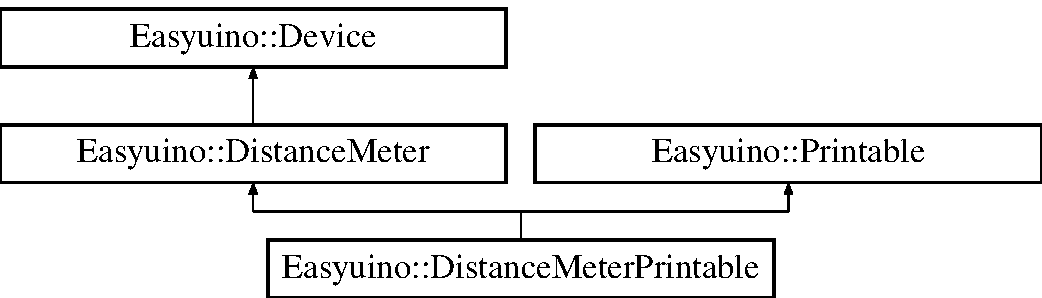
\includegraphics[height=3.000000cm]{class_easyuino_1_1_distance_meter_printable}
\end{center}
\end{figure}
\subsection*{Public Member Functions}
\begin{DoxyCompactItemize}
\item 
\mbox{\Hypertarget{class_easyuino_1_1_distance_meter_printable_a367fe13996801c142f687234390bfc8c}\label{class_easyuino_1_1_distance_meter_printable_a367fe13996801c142f687234390bfc8c}} 
{\bfseries Distance\+Meter\+Printable} (IN uint8\+\_\+t trigger\+Pin, IN uint8\+\_\+t echo\+Pin)
\item 
\mbox{\Hypertarget{class_easyuino_1_1_distance_meter_printable_a42bb42319353c84294975ed5edc3a84c}\label{class_easyuino_1_1_distance_meter_printable_a42bb42319353c84294975ed5edc3a84c}} 
char $\ast$ {\bfseries to\+String} () const
\end{DoxyCompactItemize}
\subsection*{Additional Inherited Members}


The documentation for this class was generated from the following file\+:\begin{DoxyCompactItemize}
\item 
src/Distance\+Meter\+Printable.\+h\end{DoxyCompactItemize}

\hypertarget{class_easyuino_1_1_g_s_m_service}{}\section{Easyuino\+:\+:G\+S\+M\+Service Class Reference}
\label{class_easyuino_1_1_g_s_m_service}\index{Easyuino\+::\+G\+S\+M\+Service@{Easyuino\+::\+G\+S\+M\+Service}}
Inheritance diagram for Easyuino\+:\+:G\+S\+M\+Service\+:\begin{figure}[H]
\begin{center}
\leavevmode
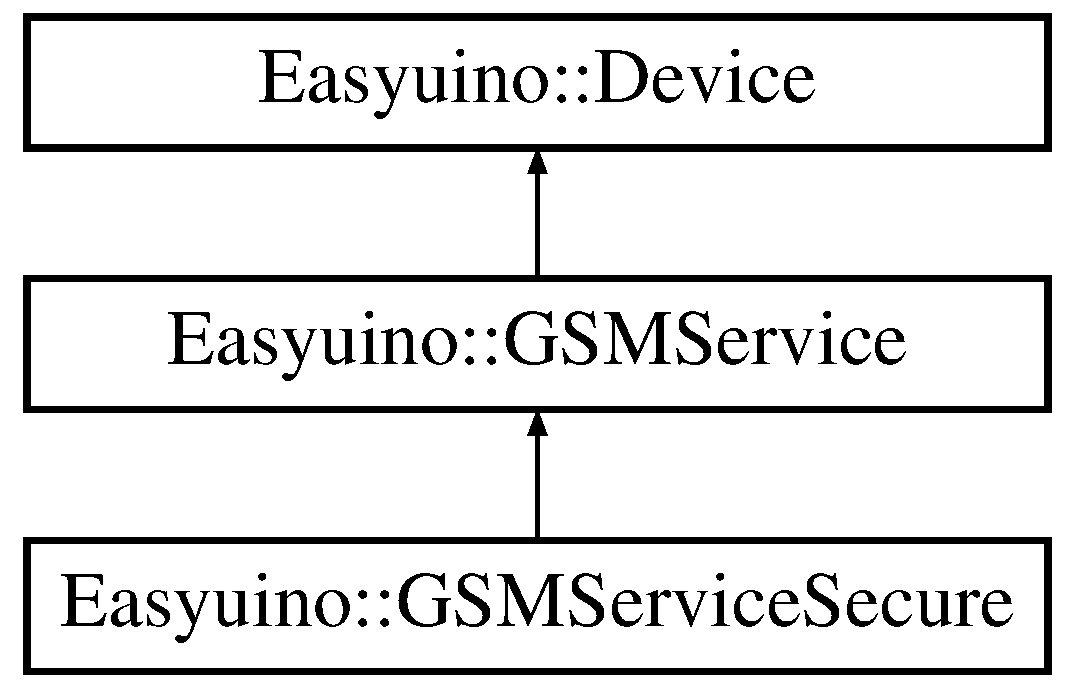
\includegraphics[height=3.000000cm]{class_easyuino_1_1_g_s_m_service}
\end{center}
\end{figure}
\subsection*{Public Member Functions}
\begin{DoxyCompactItemize}
\item 
\mbox{\Hypertarget{class_easyuino_1_1_g_s_m_service_ad8700c921a8f3ce267369e9843853be1}\label{class_easyuino_1_1_g_s_m_service_ad8700c921a8f3ce267369e9843853be1}} 
{\bfseries G\+S\+M\+Service} (IN uint8\+\_\+t tx\+Pin, IN uint8\+\_\+t rx\+Pin, IN uint8\+\_\+t power\+Pin, IN Stream \&output\+Stream)
\item 
\mbox{\Hypertarget{class_easyuino_1_1_g_s_m_service_ab856f1ecdb47de6b13f186bea7c69ce2}\label{class_easyuino_1_1_g_s_m_service_ab856f1ecdb47de6b13f186bea7c69ce2}} 
{\bfseries G\+S\+M\+Service} (IN uint8\+\_\+t tx\+Pin, IN uint8\+\_\+t rx\+Pin, IN uint8\+\_\+t power\+Pin)
\item 
\mbox{\Hypertarget{class_easyuino_1_1_g_s_m_service_a49dd695dba030b168464f620c3d96ee0}\label{class_easyuino_1_1_g_s_m_service_a49dd695dba030b168464f620c3d96ee0}} 
bool {\bfseries begin} (IN unsigned long gsm\+Module\+Baud\+Rate)
\item 
bool \hyperlink{class_easyuino_1_1_g_s_m_service_aeafc2dae47e4b13e127eb228a0f7ff6a}{begin} ()
\begin{DoxyCompactList}\small\item\em Used to put the device ready to receive requests. \end{DoxyCompactList}\item 
void \hyperlink{class_easyuino_1_1_g_s_m_service_a05bef783773776ec209608aa81d1ff45}{end} ()
\begin{DoxyCompactList}\small\item\em Used to stop the device A\+PI. \end{DoxyCompactList}\item 
\mbox{\Hypertarget{class_easyuino_1_1_g_s_m_service_ad5bd54c7dfcc402df0fac92c88e07c6e}\label{class_easyuino_1_1_g_s_m_service_ad5bd54c7dfcc402df0fac92c88e07c6e}} 
G\+S\+M\+Request\+Status {\bfseries turn\+On} ()
\item 
\mbox{\Hypertarget{class_easyuino_1_1_g_s_m_service_a327c2610c2aa7ba5a54530d87a0d6128}\label{class_easyuino_1_1_g_s_m_service_a327c2610c2aa7ba5a54530d87a0d6128}} 
G\+S\+M\+Request\+Status {\bfseries turn\+Off} ()
\item 
\mbox{\Hypertarget{class_easyuino_1_1_g_s_m_service_a2ad440efbd04942d956212988d20a0df}\label{class_easyuino_1_1_g_s_m_service_a2ad440efbd04942d956212988d20a0df}} 
G\+S\+M\+Request\+Status {\bfseries is\+On} (O\+UT bool \&result)
\item 
\mbox{\Hypertarget{class_easyuino_1_1_g_s_m_service_a6b6ee723ceaf62bfd9312278b5dbf36d}\label{class_easyuino_1_1_g_s_m_service_a6b6ee723ceaf62bfd9312278b5dbf36d}} 
G\+S\+M\+Request\+Status {\bfseries set\+Baud\+Rate} (IN unsigned long new\+Baud\+Rate)
\item 
\mbox{\Hypertarget{class_easyuino_1_1_g_s_m_service_a8fd764ef215a16f676e6e5e4b283b61d}\label{class_easyuino_1_1_g_s_m_service_a8fd764ef215a16f676e6e5e4b283b61d}} 
G\+S\+M\+Request\+Status {\bfseries begin\+Listen\+For\+S\+MS} ()
\item 
\mbox{\Hypertarget{class_easyuino_1_1_g_s_m_service_a02c2bddace1c87f035f324ae248c4f1d}\label{class_easyuino_1_1_g_s_m_service_a02c2bddace1c87f035f324ae248c4f1d}} 
virtual G\+S\+M\+Request\+Status {\bfseries available\+S\+MS} (O\+UT \hyperlink{class_easyuino_1_1_s_m_s}{S\+MS} \&message, O\+UT bool \&sms\+Read)
\item 
\mbox{\Hypertarget{class_easyuino_1_1_g_s_m_service_ae860cc330ef552c733d9ab4a5c2fd366}\label{class_easyuino_1_1_g_s_m_service_ae860cc330ef552c733d9ab4a5c2fd366}} 
G\+S\+M\+Request\+Status {\bfseries send\+S\+MS} (IN \hyperlink{class_easyuino_1_1_s_m_s}{S\+MS} \&sms)
\item 
\mbox{\Hypertarget{class_easyuino_1_1_g_s_m_service_ad37d83f2a91fbe2e50a11f1d435eccb5}\label{class_easyuino_1_1_g_s_m_service_ad37d83f2a91fbe2e50a11f1d435eccb5}} 
G\+S\+M\+Request\+Status {\bfseries send\+S\+MS} (IN unsigned long phone\+Number, IN const char $\ast$message, IN unsigned int country\+Prefix\+Code)
\item 
\mbox{\Hypertarget{class_easyuino_1_1_g_s_m_service_aef4379e7c82f275f0af341f79a3b451f}\label{class_easyuino_1_1_g_s_m_service_aef4379e7c82f275f0af341f79a3b451f}} 
G\+S\+M\+Request\+Status {\bfseries delete\+All\+S\+MS} ()
\item 
\mbox{\Hypertarget{class_easyuino_1_1_g_s_m_service_af142e4f7d99cffda9a3598446466cdb3}\label{class_easyuino_1_1_g_s_m_service_af142e4f7d99cffda9a3598446466cdb3}} 
G\+S\+M\+Request\+Status {\bfseries delete\+All\+Read\+S\+MS} ()
\item 
\mbox{\Hypertarget{class_easyuino_1_1_g_s_m_service_a7b457ab0669a8e9c16ab1906cc246365}\label{class_easyuino_1_1_g_s_m_service_a7b457ab0669a8e9c16ab1906cc246365}} 
G\+S\+M\+Request\+Status {\bfseries delete\+All\+Sent\+And\+Read\+S\+MS} ()
\end{DoxyCompactItemize}
\subsection*{Additional Inherited Members}


\subsection{Member Function Documentation}
\mbox{\Hypertarget{class_easyuino_1_1_g_s_m_service_aeafc2dae47e4b13e127eb228a0f7ff6a}\label{class_easyuino_1_1_g_s_m_service_aeafc2dae47e4b13e127eb228a0f7ff6a}} 
\index{Easyuino\+::\+G\+S\+M\+Service@{Easyuino\+::\+G\+S\+M\+Service}!begin@{begin}}
\index{begin@{begin}!Easyuino\+::\+G\+S\+M\+Service@{Easyuino\+::\+G\+S\+M\+Service}}
\subsubsection{\texorpdfstring{begin()}{begin()}}
{\footnotesize\ttfamily bool Easyuino\+::\+G\+S\+M\+Service\+::begin (\begin{DoxyParamCaption}{ }\end{DoxyParamCaption})\hspace{0.3cm}{\ttfamily [virtual]}}



Used to put the device ready to receive requests. 

Normally this have some default behaviour some devices have other overload method with same name that receives other arguments to device customization. \begin{DoxyReturn}{Returns}
True\+: If the device was initialized. False\+: Otherwise. 
\end{DoxyReturn}


Implements \hyperlink{class_easyuino_1_1_device_a2e7bb2fec849719a9d9432b57cdb72ba}{Easyuino\+::\+Device}.

\mbox{\Hypertarget{class_easyuino_1_1_g_s_m_service_a05bef783773776ec209608aa81d1ff45}\label{class_easyuino_1_1_g_s_m_service_a05bef783773776ec209608aa81d1ff45}} 
\index{Easyuino\+::\+G\+S\+M\+Service@{Easyuino\+::\+G\+S\+M\+Service}!end@{end}}
\index{end@{end}!Easyuino\+::\+G\+S\+M\+Service@{Easyuino\+::\+G\+S\+M\+Service}}
\subsubsection{\texorpdfstring{end()}{end()}}
{\footnotesize\ttfamily void Easyuino\+::\+G\+S\+M\+Service\+::end (\begin{DoxyParamCaption}{ }\end{DoxyParamCaption})\hspace{0.3cm}{\ttfamily [virtual]}}



Used to stop the device A\+PI. 

After this the the device will not process A\+PI requests. 

Implements \hyperlink{class_easyuino_1_1_device_ab31018ef64adc84aa2ea575b2297548f}{Easyuino\+::\+Device}.



The documentation for this class was generated from the following file\+:\begin{DoxyCompactItemize}
\item 
src/G\+S\+M\+Service.\+h\end{DoxyCompactItemize}

\hypertarget{class_easyuino_1_1_g_s_m_service_secure}{}\section{Easyuino\+:\+:G\+S\+M\+Service\+Secure Class Reference}
\label{class_easyuino_1_1_g_s_m_service_secure}\index{Easyuino\+::\+G\+S\+M\+Service\+Secure@{Easyuino\+::\+G\+S\+M\+Service\+Secure}}
Inheritance diagram for Easyuino\+:\+:G\+S\+M\+Service\+Secure\+:\begin{figure}[H]
\begin{center}
\leavevmode
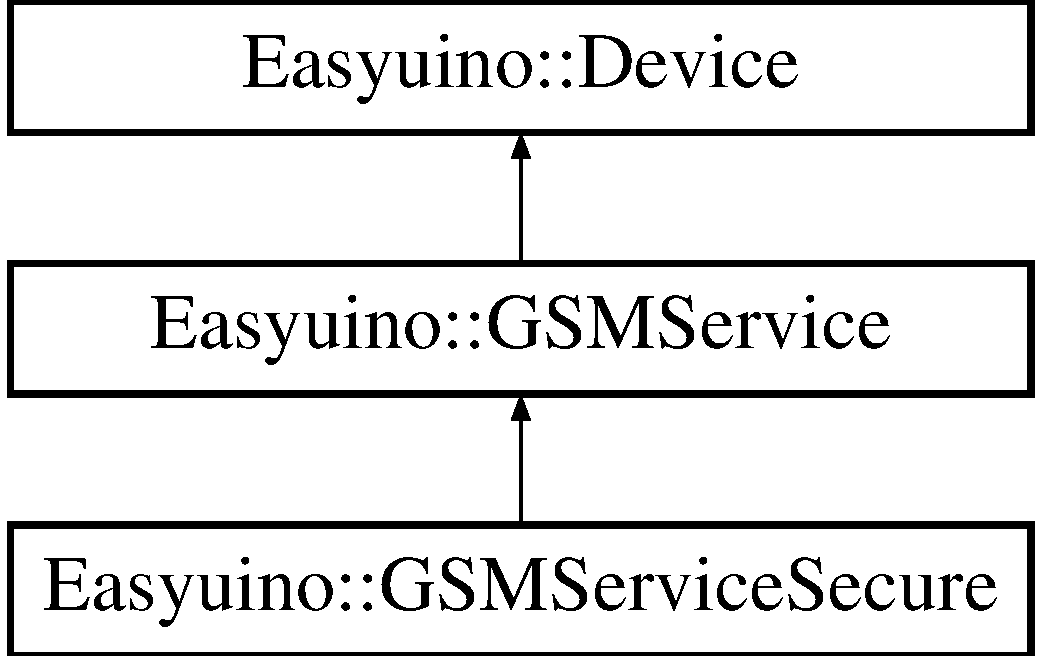
\includegraphics[height=3.000000cm]{class_easyuino_1_1_g_s_m_service_secure}
\end{center}
\end{figure}
\subsection*{Public Member Functions}
\begin{DoxyCompactItemize}
\item 
\mbox{\Hypertarget{class_easyuino_1_1_g_s_m_service_secure_ab28bad6e7765f61851a3957edc5d3071}\label{class_easyuino_1_1_g_s_m_service_secure_ab28bad6e7765f61851a3957edc5d3071}} 
{\bfseries G\+S\+M\+Service\+Secure} (IN uint8\+\_\+t tx\+Pin, IN uint8\+\_\+t rx\+Pin, IN uint8\+\_\+t power\+Pin, IN Stream \&output\+Stream)
\item 
\mbox{\Hypertarget{class_easyuino_1_1_g_s_m_service_secure_a4331122e2c6e42711eb13bf59cfd940c}\label{class_easyuino_1_1_g_s_m_service_secure_a4331122e2c6e42711eb13bf59cfd940c}} 
{\bfseries G\+S\+M\+Service\+Secure} (IN uint8\+\_\+t tx\+Pin, IN uint8\+\_\+t rx\+Pin, IN uint8\+\_\+t power\+Pin)
\item 
\mbox{\Hypertarget{class_easyuino_1_1_g_s_m_service_secure_a7acbf1d460ef1b81bcd36d852b596af3}\label{class_easyuino_1_1_g_s_m_service_secure_a7acbf1d460ef1b81bcd36d852b596af3}} 
G\+S\+M\+Request\+Status {\bfseries add\+Allowed\+Number} (IN unsigned long phone\+Number\+To\+Add)
\item 
\mbox{\Hypertarget{class_easyuino_1_1_g_s_m_service_secure_a791dd872fe2c72311d84219616e5f54c}\label{class_easyuino_1_1_g_s_m_service_secure_a791dd872fe2c72311d84219616e5f54c}} 
G\+S\+M\+Request\+Status {\bfseries is\+Allowed} (IN unsigned long phone\+Number, O\+UT bool \&allowed)
\item 
\mbox{\Hypertarget{class_easyuino_1_1_g_s_m_service_secure_a1ad4988fa2dcc0ba8f87c70cf71edf29}\label{class_easyuino_1_1_g_s_m_service_secure_a1ad4988fa2dcc0ba8f87c70cf71edf29}} 
G\+S\+M\+Request\+Status {\bfseries remove\+Allowed\+Number} (IN unsigned long phone\+Number\+To\+Remove)
\item 
\mbox{\Hypertarget{class_easyuino_1_1_g_s_m_service_secure_a10a8160dfb473d84b4bd182d689bdb95}\label{class_easyuino_1_1_g_s_m_service_secure_a10a8160dfb473d84b4bd182d689bdb95}} 
G\+S\+M\+Request\+Status {\bfseries clear\+Allowed\+Numbers} ()
\item 
\mbox{\Hypertarget{class_easyuino_1_1_g_s_m_service_secure_a6c64fcfd9f98bec206543bc1699623d7}\label{class_easyuino_1_1_g_s_m_service_secure_a6c64fcfd9f98bec206543bc1699623d7}} 
virtual G\+S\+M\+Request\+Status {\bfseries available\+S\+MS} (I\+N\+O\+UT \hyperlink{class_easyuino_1_1_s_m_s}{S\+MS} \&message, O\+UT bool \&sms\+Read)
\end{DoxyCompactItemize}
\subsection*{Additional Inherited Members}


The documentation for this class was generated from the following file\+:\begin{DoxyCompactItemize}
\item 
src/G\+S\+M\+Service\+Secure.\+h\end{DoxyCompactItemize}

\hypertarget{class_easyuino_1_1_infra_red_receiver}{}\section{Easyuino\+:\+:Infra\+Red\+Receiver Class Reference}
\label{class_easyuino_1_1_infra_red_receiver}\index{Easyuino\+::\+Infra\+Red\+Receiver@{Easyuino\+::\+Infra\+Red\+Receiver}}
Inheritance diagram for Easyuino\+:\+:Infra\+Red\+Receiver\+:\begin{figure}[H]
\begin{center}
\leavevmode
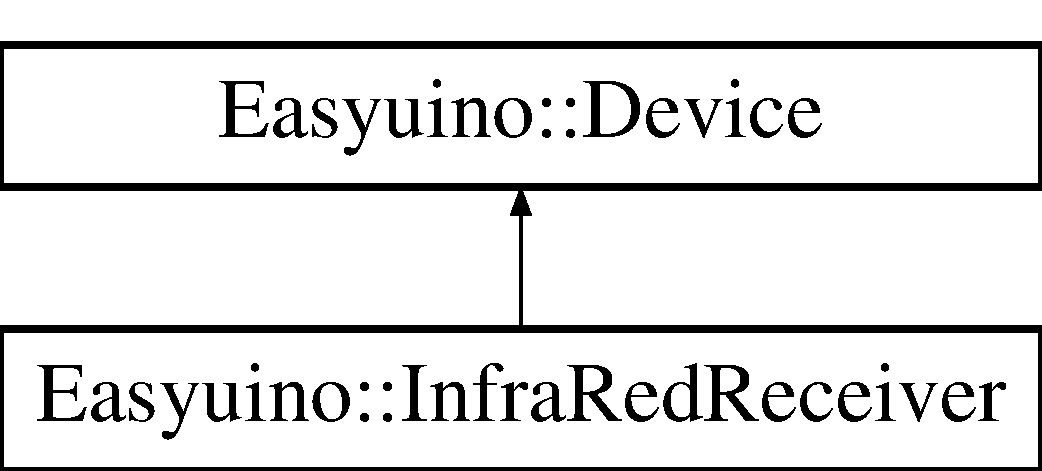
\includegraphics[height=2.000000cm]{class_easyuino_1_1_infra_red_receiver}
\end{center}
\end{figure}
\subsection*{Additional Inherited Members}


The documentation for this class was generated from the following file\+:\begin{DoxyCompactItemize}
\item 
src/Infra\+Red\+Receiver.\+h\end{DoxyCompactItemize}

\hypertarget{class_easyuino_1_1_printable}{}\section{Easyuino\+:\+:Printable Class Reference}
\label{class_easyuino_1_1_printable}\index{Easyuino\+::\+Printable@{Easyuino\+::\+Printable}}
Inheritance diagram for Easyuino\+:\+:Printable\+:\begin{figure}[H]
\begin{center}
\leavevmode
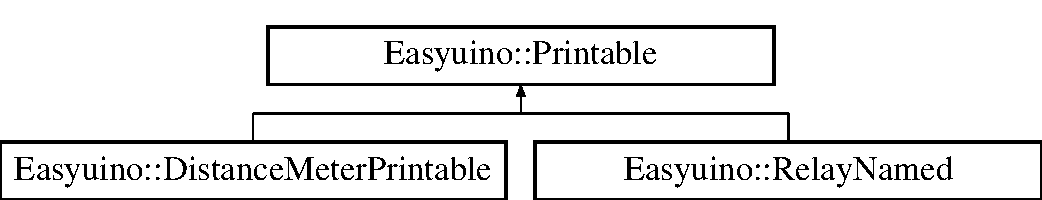
\includegraphics[height=2.000000cm]{class_easyuino_1_1_printable}
\end{center}
\end{figure}
\subsection*{Public Member Functions}
\begin{DoxyCompactItemize}
\item 
\mbox{\Hypertarget{class_easyuino_1_1_printable_a49ae1c60dc0404600ee122c6c2684155}\label{class_easyuino_1_1_printable_a49ae1c60dc0404600ee122c6c2684155}} 
virtual char $\ast$ {\bfseries to\+String} () const =0
\end{DoxyCompactItemize}
\subsection*{Friends}
\begin{DoxyCompactItemize}
\item 
\mbox{\Hypertarget{class_easyuino_1_1_printable_a50c7f93c6a84fde9f1f97f1185d853d9}\label{class_easyuino_1_1_printable_a50c7f93c6a84fde9f1f97f1185d853d9}} 
Stream \& {\bfseries operator$<$$<$} (IN Stream \&stream, IN const \hyperlink{class_easyuino_1_1_printable}{Printable} \&printable)
\end{DoxyCompactItemize}


The documentation for this class was generated from the following file\+:\begin{DoxyCompactItemize}
\item 
src/Printable.\+h\end{DoxyCompactItemize}

\hypertarget{class_easyuino_1_1_relay}{}\section{Easyuino\+:\+:Relay Class Reference}
\label{class_easyuino_1_1_relay}\index{Easyuino\+::\+Relay@{Easyuino\+::\+Relay}}


\hyperlink{class_easyuino_1_1_relay}{Relay} offers a simple A\+PI to interact with relay devices.  




{\ttfamily \#include $<$Relay.\+h$>$}

Inheritance diagram for Easyuino\+:\+:Relay\+:\begin{figure}[H]
\begin{center}
\leavevmode
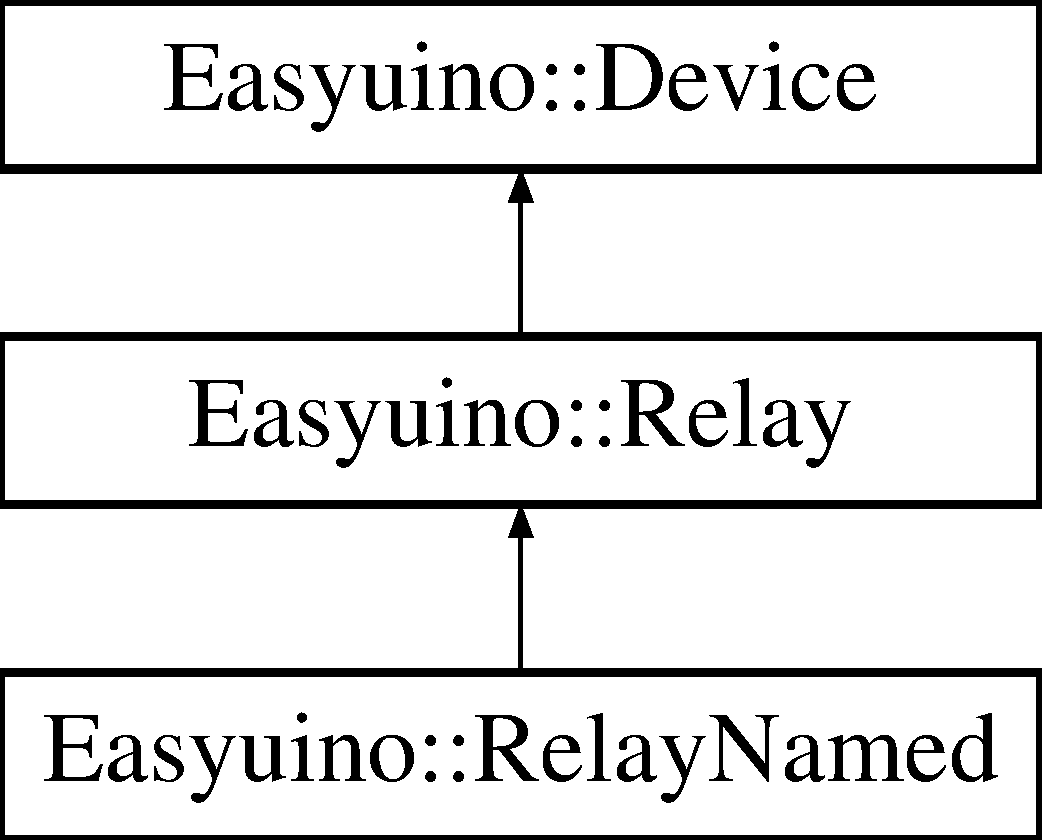
\includegraphics[height=3.000000cm]{class_easyuino_1_1_relay}
\end{center}
\end{figure}
\subsection*{Public Member Functions}
\begin{DoxyCompactItemize}
\item 
\hyperlink{class_easyuino_1_1_relay_a34a9e8461a4018e88ee49d956aca37f7}{Relay} (IN uint8\+\_\+t arduino\+Pin)
\begin{DoxyCompactList}\small\item\em Constructor. \end{DoxyCompactList}\item 
\mbox{\Hypertarget{class_easyuino_1_1_relay_a05bb65f34a842d8b044d2f8d81c2f622}\label{class_easyuino_1_1_relay_a05bb65f34a842d8b044d2f8d81c2f622}} 
\hyperlink{class_easyuino_1_1_relay_a05bb65f34a842d8b044d2f8d81c2f622}{$\sim$\+Relay} ()
\begin{DoxyCompactList}\small\item\em Destructor. \end{DoxyCompactList}\item 
bool \hyperlink{class_easyuino_1_1_relay_a920a0fa287cacfd8c6df19d8812d4958}{begin} ()
\begin{DoxyCompactList}\small\item\em Used to put the device ready to receive requests. \end{DoxyCompactList}\item 
bool \hyperlink{class_easyuino_1_1_relay_a05e66468ee1b991f394d9182b9886bf7}{begin} (IN bool is\+Normally\+Closed, IN uint8\+\_\+t normally\+Closed\+Pin\+Level)
\begin{DoxyCompactList}\small\item\em Used to initialize the relay A\+PI depending on how the relay will be connected. \end{DoxyCompactList}\item 
void \hyperlink{class_easyuino_1_1_relay_a2b57237c996a6ffe8e900ae273bce9d4}{end} ()
\begin{DoxyCompactList}\small\item\em Used to stop the device A\+PI. \end{DoxyCompactList}\item 
\mbox{\Hypertarget{class_easyuino_1_1_relay_a28b594b3ee957e062630fa2c771a966d}\label{class_easyuino_1_1_relay_a28b594b3ee957e062630fa2c771a966d}} 
void \hyperlink{class_easyuino_1_1_relay_a28b594b3ee957e062630fa2c771a966d}{turn\+On} ()
\begin{DoxyCompactList}\small\item\em Turns on the device that is connected to the relay (depends on how the begin(bool,uint8\+\_\+t) was called) \end{DoxyCompactList}\item 
\mbox{\Hypertarget{class_easyuino_1_1_relay_a9cab51ad0aaea32752df829f3f6b8113}\label{class_easyuino_1_1_relay_a9cab51ad0aaea32752df829f3f6b8113}} 
void \hyperlink{class_easyuino_1_1_relay_a9cab51ad0aaea32752df829f3f6b8113}{turn\+Off} ()
\begin{DoxyCompactList}\small\item\em Turns off the device that is connected to the relay (depends on how the begin(bool,uint8\+\_\+t) was called) \end{DoxyCompactList}\item 
bool \hyperlink{class_easyuino_1_1_relay_af8b4ac99e27ffac6c5f8d69d36dc01f5}{is\+On} () const
\end{DoxyCompactItemize}
\subsection*{Additional Inherited Members}


\subsection{Detailed Description}
\hyperlink{class_easyuino_1_1_relay}{Relay} offers a simple A\+PI to interact with relay devices. 

\begin{DoxySeeAlso}{See also}
Devices Supported\+: S\+R\+D-\/05\+V\+D\+C-\/\+S\+L-\/C, Probably any relay because they are very simple devices 

Devices Tested\+: S\+R\+D-\/05\+V\+D\+C-\/\+S\+L-\/C 
\end{DoxySeeAlso}


\subsection{Constructor \& Destructor Documentation}
\mbox{\Hypertarget{class_easyuino_1_1_relay_a34a9e8461a4018e88ee49d956aca37f7}\label{class_easyuino_1_1_relay_a34a9e8461a4018e88ee49d956aca37f7}} 
\index{Easyuino\+::\+Relay@{Easyuino\+::\+Relay}!Relay@{Relay}}
\index{Relay@{Relay}!Easyuino\+::\+Relay@{Easyuino\+::\+Relay}}
\subsubsection{\texorpdfstring{Relay()}{Relay()}}
{\footnotesize\ttfamily Easyuino\+::\+Relay\+::\+Relay (\begin{DoxyParamCaption}\item[{IN uint8\+\_\+t}]{arduino\+Pin }\end{DoxyParamCaption})}



Constructor. 


\begin{DoxyParams}{Parameters}
{\em arduino\+Pin} & Arduino pin that is connected with the relay (normaly called IN pins in the relay boards) \\
\hline
\end{DoxyParams}


\subsection{Member Function Documentation}
\mbox{\Hypertarget{class_easyuino_1_1_relay_a920a0fa287cacfd8c6df19d8812d4958}\label{class_easyuino_1_1_relay_a920a0fa287cacfd8c6df19d8812d4958}} 
\index{Easyuino\+::\+Relay@{Easyuino\+::\+Relay}!begin@{begin}}
\index{begin@{begin}!Easyuino\+::\+Relay@{Easyuino\+::\+Relay}}
\subsubsection{\texorpdfstring{begin()}{begin()}\hspace{0.1cm}{\footnotesize\ttfamily [1/2]}}
{\footnotesize\ttfamily bool Easyuino\+::\+Relay\+::begin (\begin{DoxyParamCaption}{ }\end{DoxyParamCaption})\hspace{0.3cm}{\ttfamily [virtual]}}



Used to put the device ready to receive requests. 

Normally this have some default behaviour some devices have other overload method with same name that receives other arguments to device customization. \begin{DoxyReturn}{Returns}
True\+: If the device was initialized. False\+: Otherwise. 
\end{DoxyReturn}


Implements \hyperlink{class_easyuino_1_1_device_a2e7bb2fec849719a9d9432b57cdb72ba}{Easyuino\+::\+Device}.

\mbox{\Hypertarget{class_easyuino_1_1_relay_a05e66468ee1b991f394d9182b9886bf7}\label{class_easyuino_1_1_relay_a05e66468ee1b991f394d9182b9886bf7}} 
\index{Easyuino\+::\+Relay@{Easyuino\+::\+Relay}!begin@{begin}}
\index{begin@{begin}!Easyuino\+::\+Relay@{Easyuino\+::\+Relay}}
\subsubsection{\texorpdfstring{begin()}{begin()}\hspace{0.1cm}{\footnotesize\ttfamily [2/2]}}
{\footnotesize\ttfamily bool Easyuino\+::\+Relay\+::begin (\begin{DoxyParamCaption}\item[{IN bool}]{is\+Normally\+Closed,  }\item[{IN uint8\+\_\+t}]{normally\+Closed\+Pin\+Level }\end{DoxyParamCaption})}



Used to initialize the relay A\+PI depending on how the relay will be connected. 


\begin{DoxyParams}{Parameters}
{\em is\+Normally\+Closed} & Define what are the state that relay is powering the device (lamp, engine, etc) Normally Closed or Normally Open \\
\hline
{\em normally\+Closed\+Pin\+Level} & Digital level of the normally closed relay state (some relays activate on H\+I\+GH other on L\+OW) \\
\hline
\end{DoxyParams}
\mbox{\Hypertarget{class_easyuino_1_1_relay_a2b57237c996a6ffe8e900ae273bce9d4}\label{class_easyuino_1_1_relay_a2b57237c996a6ffe8e900ae273bce9d4}} 
\index{Easyuino\+::\+Relay@{Easyuino\+::\+Relay}!end@{end}}
\index{end@{end}!Easyuino\+::\+Relay@{Easyuino\+::\+Relay}}
\subsubsection{\texorpdfstring{end()}{end()}}
{\footnotesize\ttfamily void Easyuino\+::\+Relay\+::end (\begin{DoxyParamCaption}{ }\end{DoxyParamCaption})\hspace{0.3cm}{\ttfamily [virtual]}}



Used to stop the device A\+PI. 

After this the the device will not process A\+PI requests. 

Implements \hyperlink{class_easyuino_1_1_device_ab31018ef64adc84aa2ea575b2297548f}{Easyuino\+::\+Device}.

\mbox{\Hypertarget{class_easyuino_1_1_relay_af8b4ac99e27ffac6c5f8d69d36dc01f5}\label{class_easyuino_1_1_relay_af8b4ac99e27ffac6c5f8d69d36dc01f5}} 
\index{Easyuino\+::\+Relay@{Easyuino\+::\+Relay}!is\+On@{is\+On}}
\index{is\+On@{is\+On}!Easyuino\+::\+Relay@{Easyuino\+::\+Relay}}
\subsubsection{\texorpdfstring{is\+On()}{isOn()}}
{\footnotesize\ttfamily bool Easyuino\+::\+Relay\+::is\+On (\begin{DoxyParamCaption}{ }\end{DoxyParamCaption}) const}

\begin{DoxyReturn}{Returns}
is\+ON True\+: If it is in open state. False\+: Otherwise. 
\end{DoxyReturn}


The documentation for this class was generated from the following file\+:\begin{DoxyCompactItemize}
\item 
src/Relay.\+h\end{DoxyCompactItemize}

\hypertarget{class_easyuino_1_1_relay_named}{}\section{Easyuino\+:\+:Relay\+Named Class Reference}
\label{class_easyuino_1_1_relay_named}\index{Easyuino\+::\+Relay\+Named@{Easyuino\+::\+Relay\+Named}}


\hyperlink{class_easyuino_1_1_relay_named}{Relay\+Named} offers the same A\+PI of the \hyperlink{class_easyuino_1_1_relay}{Relay} plus the possibility to associate a string label to the A\+PI object.  




{\ttfamily \#include $<$Relay\+Named.\+h$>$}

Inheritance diagram for Easyuino\+:\+:Relay\+Named\+:\begin{figure}[H]
\begin{center}
\leavevmode
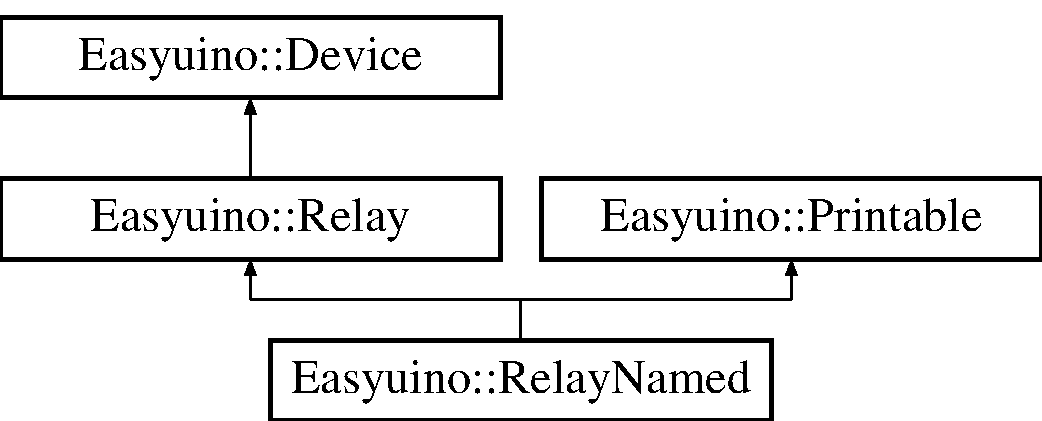
\includegraphics[height=3.000000cm]{class_easyuino_1_1_relay_named}
\end{center}
\end{figure}
\subsection*{Public Member Functions}
\begin{DoxyCompactItemize}
\item 
\hyperlink{class_easyuino_1_1_relay_named_a3def4eb321085beb48fa3e45da5e6dfc}{Relay\+Named} (IN uint8\+\_\+t arduino\+Pin, IN const char $\ast$device\+Name)
\begin{DoxyCompactList}\small\item\em Constructor. \end{DoxyCompactList}\item 
char $\ast$ \hyperlink{class_easyuino_1_1_relay_named_a1e9e82e563baaba5055ee9335551a306}{to\+String} () const
\begin{DoxyCompactList}\small\item\em Used to return a string representation of the object state. \end{DoxyCompactList}\end{DoxyCompactItemize}
\subsection*{Additional Inherited Members}


\subsection{Detailed Description}
\hyperlink{class_easyuino_1_1_relay_named}{Relay\+Named} offers the same A\+PI of the \hyperlink{class_easyuino_1_1_relay}{Relay} plus the possibility to associate a string label to the A\+PI object. 

\begin{DoxySeeAlso}{See also}
Devices Supported\+: S\+R\+D-\/05\+V\+D\+C-\/\+S\+L-\/C, Probably any relay because they are very simple devices 

Devices Tested\+: S\+R\+D-\/05\+V\+D\+C-\/\+S\+L-\/C 
\end{DoxySeeAlso}


\subsection{Constructor \& Destructor Documentation}
\mbox{\Hypertarget{class_easyuino_1_1_relay_named_a3def4eb321085beb48fa3e45da5e6dfc}\label{class_easyuino_1_1_relay_named_a3def4eb321085beb48fa3e45da5e6dfc}} 
\index{Easyuino\+::\+Relay\+Named@{Easyuino\+::\+Relay\+Named}!Relay\+Named@{Relay\+Named}}
\index{Relay\+Named@{Relay\+Named}!Easyuino\+::\+Relay\+Named@{Easyuino\+::\+Relay\+Named}}
\subsubsection{\texorpdfstring{Relay\+Named()}{RelayNamed()}}
{\footnotesize\ttfamily Easyuino\+::\+Relay\+Named\+::\+Relay\+Named (\begin{DoxyParamCaption}\item[{IN uint8\+\_\+t}]{arduino\+Pin,  }\item[{IN const char $\ast$}]{device\+Name }\end{DoxyParamCaption})}



Constructor. 


\begin{DoxyParams}{Parameters}
{\em arduino\+Pin} & Arduino pin that is connected with the relay (normal in relay is IN pins) \\
\hline
{\em device\+Name} & Name (identifier) of the device that the relay activates/deactivates \\
\hline
\end{DoxyParams}


\subsection{Member Function Documentation}
\mbox{\Hypertarget{class_easyuino_1_1_relay_named_a1e9e82e563baaba5055ee9335551a306}\label{class_easyuino_1_1_relay_named_a1e9e82e563baaba5055ee9335551a306}} 
\index{Easyuino\+::\+Relay\+Named@{Easyuino\+::\+Relay\+Named}!to\+String@{to\+String}}
\index{to\+String@{to\+String}!Easyuino\+::\+Relay\+Named@{Easyuino\+::\+Relay\+Named}}
\subsubsection{\texorpdfstring{to\+String()}{toString()}}
{\footnotesize\ttfamily char$\ast$ Easyuino\+::\+Relay\+Named\+::to\+String (\begin{DoxyParamCaption}{ }\end{DoxyParamCaption}) const\hspace{0.3cm}{\ttfamily [virtual]}}



Used to return a string representation of the object state. 

I\+M\+P\+O\+R\+T\+A\+NT\+: It is mandatory to free the returned pointer in order to have no memory leaks. 

Implements \hyperlink{class_easyuino_1_1_printable_a49ae1c60dc0404600ee122c6c2684155}{Easyuino\+::\+Printable}.



The documentation for this class was generated from the following file\+:\begin{DoxyCompactItemize}
\item 
src/Relay\+Named.\+h\end{DoxyCompactItemize}

\hypertarget{class_easyuino_1_1_r_g_b_led}{}\section{Easyuino\+:\+:R\+G\+B\+Led Class Reference}
\label{class_easyuino_1_1_r_g_b_led}\index{Easyuino\+::\+R\+G\+B\+Led@{Easyuino\+::\+R\+G\+B\+Led}}
Inheritance diagram for Easyuino\+:\+:R\+G\+B\+Led\+:\begin{figure}[H]
\begin{center}
\leavevmode
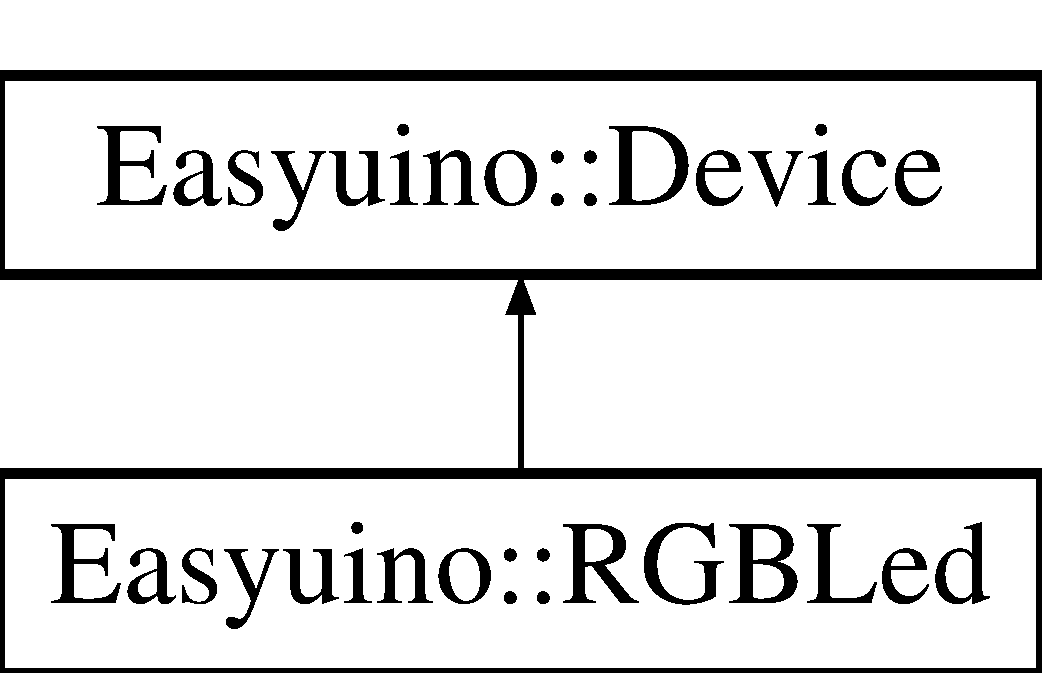
\includegraphics[height=2.000000cm]{class_easyuino_1_1_r_g_b_led}
\end{center}
\end{figure}
\subsection*{Public Member Functions}
\begin{DoxyCompactItemize}
\item 
\mbox{\Hypertarget{class_easyuino_1_1_r_g_b_led_a3580be3110cebddcd06917994ebdb8ad}\label{class_easyuino_1_1_r_g_b_led_a3580be3110cebddcd06917994ebdb8ad}} 
{\bfseries R\+G\+B\+Led} (IN uint8\+\_\+t red\+Pin, IN uint8\+\_\+t green\+Pin, IN uint8\+\_\+t blue\+Pin)
\item 
\mbox{\Hypertarget{class_easyuino_1_1_r_g_b_led_a85c5af3b8b5288d7b45eabcf4fc71aba}\label{class_easyuino_1_1_r_g_b_led_a85c5af3b8b5288d7b45eabcf4fc71aba}} 
{\bfseries R\+G\+B\+Led} (IN uint8\+\_\+t red\+Pin, IN uint8\+\_\+t green\+Pin, IN uint8\+\_\+t blue\+Pin, IN Led\+Type led\+Type)
\item 
\mbox{\Hypertarget{class_easyuino_1_1_r_g_b_led_abdc3512266c7f584609147fccc1ec816}\label{class_easyuino_1_1_r_g_b_led_abdc3512266c7f584609147fccc1ec816}} 
bool {\bfseries begin} ()
\item 
\mbox{\Hypertarget{class_easyuino_1_1_r_g_b_led_ad0e9fb0da405c537e876c8a2dc22246e}\label{class_easyuino_1_1_r_g_b_led_ad0e9fb0da405c537e876c8a2dc22246e}} 
void {\bfseries end} ()
\item 
\mbox{\Hypertarget{class_easyuino_1_1_r_g_b_led_a100140fa6d32e190f68cdc1e24c3aba0}\label{class_easyuino_1_1_r_g_b_led_a100140fa6d32e190f68cdc1e24c3aba0}} 
void {\bfseries turn\+Off} ()
\item 
\mbox{\Hypertarget{class_easyuino_1_1_r_g_b_led_a4c113ab3fbbd2a75f020a902355faa3e}\label{class_easyuino_1_1_r_g_b_led_a4c113ab3fbbd2a75f020a902355faa3e}} 
void {\bfseries set\+Color} (IN uint8\+\_\+t red, IN uint8\+\_\+t green, IN uint8\+\_\+t blue)
\item 
\mbox{\Hypertarget{class_easyuino_1_1_r_g_b_led_a66ad7b78c2ae636c077519950952206c}\label{class_easyuino_1_1_r_g_b_led_a66ad7b78c2ae636c077519950952206c}} 
void {\bfseries set\+Color} (IN char hexadecimal\+Colo\+Code\mbox{[}8\mbox{]})
\item 
\mbox{\Hypertarget{class_easyuino_1_1_r_g_b_led_a5b8365a4191bbe0a092ba30996a37b13}\label{class_easyuino_1_1_r_g_b_led_a5b8365a4191bbe0a092ba30996a37b13}} 
void {\bfseries set\+Color} (IN Color color)
\end{DoxyCompactItemize}
\subsection*{Additional Inherited Members}


The documentation for this class was generated from the following files\+:\begin{DoxyCompactItemize}
\item 
src/R\+G\+B\+Led.\+h\item 
src/main/\+Led/R\+G\+B\+Led.\+cpp\end{DoxyCompactItemize}

\hypertarget{class_easyuino_1_1_seven_segments}{}\section{Easyuino\+:\+:Seven\+Segments Class Reference}
\label{class_easyuino_1_1_seven_segments}\index{Easyuino\+::\+Seven\+Segments@{Easyuino\+::\+Seven\+Segments}}
Inheritance diagram for Easyuino\+:\+:Seven\+Segments\+:\begin{figure}[H]
\begin{center}
\leavevmode
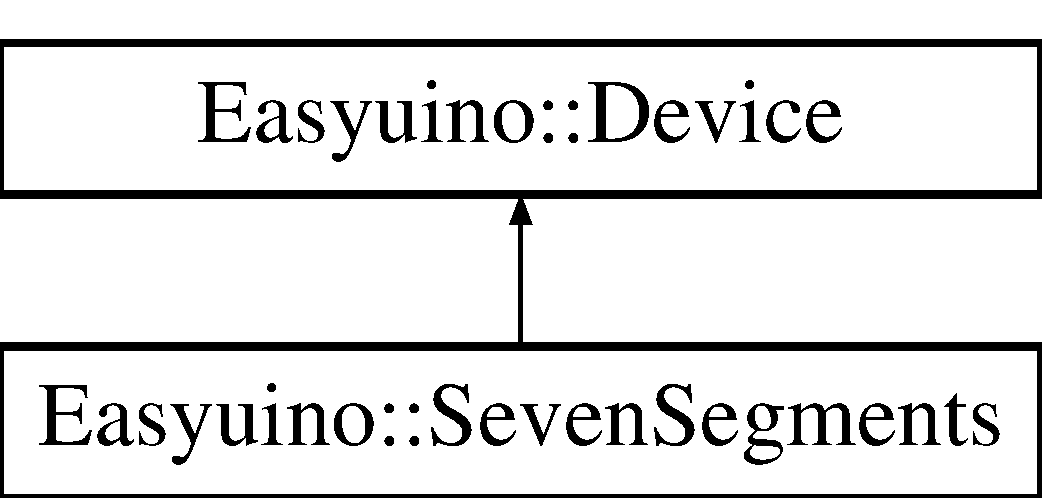
\includegraphics[height=2.000000cm]{class_easyuino_1_1_seven_segments}
\end{center}
\end{figure}
\subsection*{Public Member Functions}
\begin{DoxyCompactItemize}
\item 
\mbox{\Hypertarget{class_easyuino_1_1_seven_segments_a4a892bc5fe3f8b27cc6b7efbd31e8012}\label{class_easyuino_1_1_seven_segments_a4a892bc5fe3f8b27cc6b7efbd31e8012}} 
{\bfseries Seven\+Segments} (uint8\+\_\+t clk\+Pin, uint8\+\_\+t data\+Pin)
\item 
bool \hyperlink{class_easyuino_1_1_seven_segments_ab59d5cbdc22567fb97854f32d899e02d}{begin} ()
\begin{DoxyCompactList}\small\item\em Used to put the device ready to receive requests. \end{DoxyCompactList}\item 
void \hyperlink{class_easyuino_1_1_seven_segments_afea49385382a7b9c597b4fe42a003fee}{end} ()
\begin{DoxyCompactList}\small\item\em Used to stop the device A\+PI. \end{DoxyCompactList}\item 
\mbox{\Hypertarget{class_easyuino_1_1_seven_segments_a37d542d1ca55d2733c2f11c8efc79f0f}\label{class_easyuino_1_1_seven_segments_a37d542d1ca55d2733c2f11c8efc79f0f}} 
void {\bfseries print} (uint8\+\_\+t byte)
\end{DoxyCompactItemize}
\subsection*{Additional Inherited Members}


\subsection{Member Function Documentation}
\mbox{\Hypertarget{class_easyuino_1_1_seven_segments_ab59d5cbdc22567fb97854f32d899e02d}\label{class_easyuino_1_1_seven_segments_ab59d5cbdc22567fb97854f32d899e02d}} 
\index{Easyuino\+::\+Seven\+Segments@{Easyuino\+::\+Seven\+Segments}!begin@{begin}}
\index{begin@{begin}!Easyuino\+::\+Seven\+Segments@{Easyuino\+::\+Seven\+Segments}}
\subsubsection{\texorpdfstring{begin()}{begin()}}
{\footnotesize\ttfamily bool Easyuino\+::\+Seven\+Segments\+::begin (\begin{DoxyParamCaption}{ }\end{DoxyParamCaption})\hspace{0.3cm}{\ttfamily [virtual]}}



Used to put the device ready to receive requests. 

Normally this have some default behaviour some devices have other overload method with same name that receives other arguments to device customization. \begin{DoxyReturn}{Returns}
True\+: If the device was initialized. False\+: Otherwise. 
\end{DoxyReturn}


Implements \hyperlink{class_easyuino_1_1_device_a2e7bb2fec849719a9d9432b57cdb72ba}{Easyuino\+::\+Device}.

\mbox{\Hypertarget{class_easyuino_1_1_seven_segments_afea49385382a7b9c597b4fe42a003fee}\label{class_easyuino_1_1_seven_segments_afea49385382a7b9c597b4fe42a003fee}} 
\index{Easyuino\+::\+Seven\+Segments@{Easyuino\+::\+Seven\+Segments}!end@{end}}
\index{end@{end}!Easyuino\+::\+Seven\+Segments@{Easyuino\+::\+Seven\+Segments}}
\subsubsection{\texorpdfstring{end()}{end()}}
{\footnotesize\ttfamily void Easyuino\+::\+Seven\+Segments\+::end (\begin{DoxyParamCaption}{ }\end{DoxyParamCaption})\hspace{0.3cm}{\ttfamily [virtual]}}



Used to stop the device A\+PI. 

After this the the device will not process A\+PI requests. 

Implements \hyperlink{class_easyuino_1_1_device_ab31018ef64adc84aa2ea575b2297548f}{Easyuino\+::\+Device}.



The documentation for this class was generated from the following file\+:\begin{DoxyCompactItemize}
\item 
src/Seven\+Segments.\+h\end{DoxyCompactItemize}

\hypertarget{class_easyuino_1_1_s_m_s}{}\section{Easyuino\+:\+:S\+MS Class Reference}
\label{class_easyuino_1_1_s_m_s}\index{Easyuino\+::\+S\+MS@{Easyuino\+::\+S\+MS}}
\subsection*{Public Member Functions}
\begin{DoxyCompactItemize}
\item 
\mbox{\Hypertarget{class_easyuino_1_1_s_m_s_a5c56de204df53688169644314e8f0efe}\label{class_easyuino_1_1_s_m_s_a5c56de204df53688169644314e8f0efe}} 
{\bfseries S\+MS} (IN unsigned long number, IN const char $\ast$message, IN unsigned int country\+Prefix\+Code=351)
\item 
\mbox{\Hypertarget{class_easyuino_1_1_s_m_s_a9088a459857f18c463d3ad198bbe0abd}\label{class_easyuino_1_1_s_m_s_a9088a459857f18c463d3ad198bbe0abd}} 
{\bfseries S\+MS} (IN unsigned int country\+Prefix\+Code=351)
\item 
\mbox{\Hypertarget{class_easyuino_1_1_s_m_s_aef79317e0ee7511d85814a10aaa15e14}\label{class_easyuino_1_1_s_m_s_aef79317e0ee7511d85814a10aaa15e14}} 
unsigned int {\bfseries get\+Country\+Prefix\+Code} ()
\item 
\mbox{\Hypertarget{class_easyuino_1_1_s_m_s_a05650de23138fee2dfc1ce9a8e2b0429}\label{class_easyuino_1_1_s_m_s_a05650de23138fee2dfc1ce9a8e2b0429}} 
void {\bfseries set\+Country\+Prefix\+Code} (IN unsigned int new\+Country\+Prefix\+Code)
\item 
\mbox{\Hypertarget{class_easyuino_1_1_s_m_s_ab46be8f783d59208245e9d14d3a046d5}\label{class_easyuino_1_1_s_m_s_ab46be8f783d59208245e9d14d3a046d5}} 
unsigned long {\bfseries get\+Number} ()
\item 
\mbox{\Hypertarget{class_easyuino_1_1_s_m_s_a6d9b21c6480b7e859dfb16688090ed1c}\label{class_easyuino_1_1_s_m_s_a6d9b21c6480b7e859dfb16688090ed1c}} 
void {\bfseries set\+Number} (IN unsigned long new\+Number)
\item 
\mbox{\Hypertarget{class_easyuino_1_1_s_m_s_ac13745969d572629274ae69f3f98ab2e}\label{class_easyuino_1_1_s_m_s_ac13745969d572629274ae69f3f98ab2e}} 
const char $\ast$ {\bfseries get\+Message} ()
\item 
\mbox{\Hypertarget{class_easyuino_1_1_s_m_s_a7c0fdcb9b1a54cf025c6b98618badc21}\label{class_easyuino_1_1_s_m_s_a7c0fdcb9b1a54cf025c6b98618badc21}} 
void {\bfseries set\+Message} (IN const char $\ast$new\+Message)
\item 
\mbox{\Hypertarget{class_easyuino_1_1_s_m_s_a0f4b83fa7be59e7efa85c4d8e36ec8e3}\label{class_easyuino_1_1_s_m_s_a0f4b83fa7be59e7efa85c4d8e36ec8e3}} 
void {\bfseries reset} ()
\end{DoxyCompactItemize}


The documentation for this class was generated from the following file\+:\begin{DoxyCompactItemize}
\item 
src/S\+M\+S.\+h\end{DoxyCompactItemize}

\hypertarget{class_easyuino_1_1_utilities}{}\section{Easyuino\+:\+:Utilities Class Reference}
\label{class_easyuino_1_1_utilities}\index{Easyuino\+::\+Utilities@{Easyuino\+::\+Utilities}}
\subsection*{Static Public Member Functions}
\begin{DoxyCompactItemize}
\item 
\mbox{\Hypertarget{class_easyuino_1_1_utilities_a5a7991900cbc3f9e4cda1289ee7a7ee1}\label{class_easyuino_1_1_utilities_a5a7991900cbc3f9e4cda1289ee7a7ee1}} 
static void $\ast$ {\bfseries Easy\+Malloc} (IN unsigned int size\+In\+Bytes)
\item 
\mbox{\Hypertarget{class_easyuino_1_1_utilities_a736bd038601132c4beac24cd88340695}\label{class_easyuino_1_1_utilities_a736bd038601132c4beac24cd88340695}} 
static void {\bfseries Zero\+Buffer} (IN void $\ast$buffer, IN size\+\_\+t buffer\+Size)
\item 
\mbox{\Hypertarget{class_easyuino_1_1_utilities_a4d7f4573ee544e72da2945f18d043704}\label{class_easyuino_1_1_utilities_a4d7f4573ee544e72da2945f18d043704}} 
static void {\bfseries Override\+Last\+String\+Char} (IN char $\ast$string)
\item 
\mbox{\Hypertarget{class_easyuino_1_1_utilities_a8f5da1e6939a43f10702b16c2fdeb8e0}\label{class_easyuino_1_1_utilities_a8f5da1e6939a43f10702b16c2fdeb8e0}} 
static void {\bfseries Override\+Last\+Two\+Char} (IN char $\ast$string)
\end{DoxyCompactItemize}


The documentation for this class was generated from the following file\+:\begin{DoxyCompactItemize}
\item 
src/Utilities.\+h\end{DoxyCompactItemize}

\hypertarget{class_easyuino_1_1_water_detector}{}\section{Easyuino\+:\+:Water\+Detector Class Reference}
\label{class_easyuino_1_1_water_detector}\index{Easyuino\+::\+Water\+Detector@{Easyuino\+::\+Water\+Detector}}


Rain\+Detector A\+PI is used to detect the amount of water that is touching the sensor.  




{\ttfamily \#include $<$Water\+Detector.\+h$>$}

Inheritance diagram for Easyuino\+:\+:Water\+Detector\+:\begin{figure}[H]
\begin{center}
\leavevmode
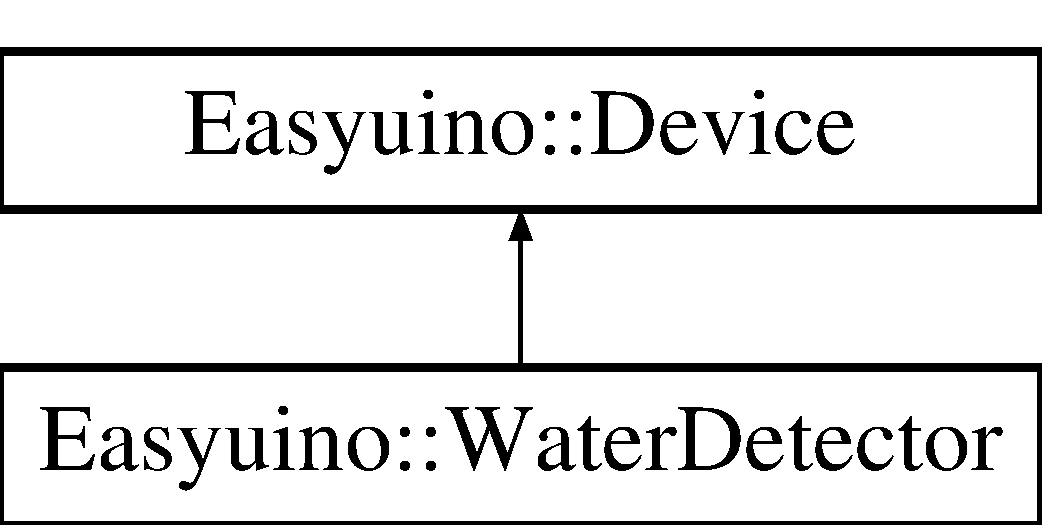
\includegraphics[height=2.000000cm]{class_easyuino_1_1_water_detector}
\end{center}
\end{figure}
\subsection*{Public Member Functions}
\begin{DoxyCompactItemize}
\item 
\hyperlink{class_easyuino_1_1_water_detector_a33690612b2b89efcfb97d4967b16c617}{Water\+Detector} (IN uint8\+\_\+t digital\+Pin, IN uint8\+\_\+t analog\+Pin)
\begin{DoxyCompactList}\small\item\em Constructor. \end{DoxyCompactList}\item 
\mbox{\Hypertarget{class_easyuino_1_1_water_detector_af63f706076f6941135412d57c1ddc5cf}\label{class_easyuino_1_1_water_detector_af63f706076f6941135412d57c1ddc5cf}} 
\hyperlink{class_easyuino_1_1_water_detector_af63f706076f6941135412d57c1ddc5cf}{$\sim$\+Water\+Detector} ()
\begin{DoxyCompactList}\small\item\em Destructor. \end{DoxyCompactList}\item 
bool \hyperlink{class_easyuino_1_1_water_detector_af7a0ec32d6abcb8c1060f493525d5228}{begin} ()
\begin{DoxyCompactList}\small\item\em Used to put the device ready to receive requests. \end{DoxyCompactList}\item 
bool \hyperlink{class_easyuino_1_1_water_detector_a06ac56298c56026691d7d6a9dbb63748}{begin} (IN uint8\+\_\+t digital\+Pin\+Trigger\+Level)
\begin{DoxyCompactList}\small\item\em Initialize the \hyperlink{class_easyuino_1_1_water_detector}{Water\+Detector} A\+PI putting it ready to receive requests. \end{DoxyCompactList}\item 
void \hyperlink{class_easyuino_1_1_water_detector_a9c1473536f47b2a7d8e1f8fb1bf5f3fd}{end} ()
\begin{DoxyCompactList}\small\item\em Used to stop the device A\+PI. \end{DoxyCompactList}\item 
Water\+Status \hyperlink{class_easyuino_1_1_water_detector_a0dfefd3b3aa2ed21f30ceb8041a8652a}{get\+Water\+Status} ()
\begin{DoxyCompactList}\small\item\em Returns an enumerate value depending on how wet is the sensor. \end{DoxyCompactList}\item 
unsigned int \hyperlink{class_easyuino_1_1_water_detector_a4a4c4a0ab6ae8a51535762f38b4f0d01}{get\+Water\+Status\+Range} ()
\begin{DoxyCompactList}\small\item\em Return a number in \mbox{[}0,1023\mbox{]} depending on dry is the sensor. \end{DoxyCompactList}\item 
bool \hyperlink{class_easyuino_1_1_water_detector_a9ea69c2eec25543fad47759379d62ce6}{is\+Water\+Detected} ()
\begin{DoxyCompactList}\small\item\em Used to get the value from the digital pin that is activated when a wet threshold is passed. \end{DoxyCompactList}\end{DoxyCompactItemize}
\subsection*{Additional Inherited Members}


\subsection{Detailed Description}
Rain\+Detector A\+PI is used to detect the amount of water that is touching the sensor. 



\subsection{Constructor \& Destructor Documentation}
\mbox{\Hypertarget{class_easyuino_1_1_water_detector_a33690612b2b89efcfb97d4967b16c617}\label{class_easyuino_1_1_water_detector_a33690612b2b89efcfb97d4967b16c617}} 
\index{Easyuino\+::\+Water\+Detector@{Easyuino\+::\+Water\+Detector}!Water\+Detector@{Water\+Detector}}
\index{Water\+Detector@{Water\+Detector}!Easyuino\+::\+Water\+Detector@{Easyuino\+::\+Water\+Detector}}
\subsubsection{\texorpdfstring{Water\+Detector()}{WaterDetector()}}
{\footnotesize\ttfamily Easyuino\+::\+Water\+Detector\+::\+Water\+Detector (\begin{DoxyParamCaption}\item[{IN uint8\+\_\+t}]{digital\+Pin,  }\item[{IN uint8\+\_\+t}]{analog\+Pin }\end{DoxyParamCaption})}



Constructor. 


\begin{DoxyParams}{Parameters}
{\em digital\+Pin} & Arduino pin connected to digital pin (Normally D0 in sensor board) \\
\hline
{\em analog\+Pin} & Arduino pin connected to analog pin (Normally A0 in sensor board) \\
\hline
\end{DoxyParams}


\subsection{Member Function Documentation}
\mbox{\Hypertarget{class_easyuino_1_1_water_detector_af7a0ec32d6abcb8c1060f493525d5228}\label{class_easyuino_1_1_water_detector_af7a0ec32d6abcb8c1060f493525d5228}} 
\index{Easyuino\+::\+Water\+Detector@{Easyuino\+::\+Water\+Detector}!begin@{begin}}
\index{begin@{begin}!Easyuino\+::\+Water\+Detector@{Easyuino\+::\+Water\+Detector}}
\subsubsection{\texorpdfstring{begin()}{begin()}\hspace{0.1cm}{\footnotesize\ttfamily [1/2]}}
{\footnotesize\ttfamily bool Easyuino\+::\+Water\+Detector\+::begin (\begin{DoxyParamCaption}{ }\end{DoxyParamCaption})\hspace{0.3cm}{\ttfamily [virtual]}}



Used to put the device ready to receive requests. 

Normally this have some default behaviour some devices have other overload method with same name that receives other arguments to device customization. \begin{DoxyReturn}{Returns}
True\+: If the device was initialized. False\+: Otherwise. 
\end{DoxyReturn}


Implements \hyperlink{class_easyuino_1_1_device_a2e7bb2fec849719a9d9432b57cdb72ba}{Easyuino\+::\+Device}.

\mbox{\Hypertarget{class_easyuino_1_1_water_detector_a06ac56298c56026691d7d6a9dbb63748}\label{class_easyuino_1_1_water_detector_a06ac56298c56026691d7d6a9dbb63748}} 
\index{Easyuino\+::\+Water\+Detector@{Easyuino\+::\+Water\+Detector}!begin@{begin}}
\index{begin@{begin}!Easyuino\+::\+Water\+Detector@{Easyuino\+::\+Water\+Detector}}
\subsubsection{\texorpdfstring{begin()}{begin()}\hspace{0.1cm}{\footnotesize\ttfamily [2/2]}}
{\footnotesize\ttfamily bool Easyuino\+::\+Water\+Detector\+::begin (\begin{DoxyParamCaption}\item[{IN uint8\+\_\+t}]{digital\+Pin\+Trigger\+Level }\end{DoxyParamCaption})}



Initialize the \hyperlink{class_easyuino_1_1_water_detector}{Water\+Detector} A\+PI putting it ready to receive requests. 


\begin{DoxyParams}{Parameters}
{\em digital\+Pin\+Trigger\+Level} & The digital level that is triggered in digital pin when water is sensed. \\
\hline
\end{DoxyParams}
\begin{DoxyReturn}{Returns}
True\+: If the device was initialized. False\+: Otherwise. 
\end{DoxyReturn}
\mbox{\Hypertarget{class_easyuino_1_1_water_detector_a9c1473536f47b2a7d8e1f8fb1bf5f3fd}\label{class_easyuino_1_1_water_detector_a9c1473536f47b2a7d8e1f8fb1bf5f3fd}} 
\index{Easyuino\+::\+Water\+Detector@{Easyuino\+::\+Water\+Detector}!end@{end}}
\index{end@{end}!Easyuino\+::\+Water\+Detector@{Easyuino\+::\+Water\+Detector}}
\subsubsection{\texorpdfstring{end()}{end()}}
{\footnotesize\ttfamily void Easyuino\+::\+Water\+Detector\+::end (\begin{DoxyParamCaption}{ }\end{DoxyParamCaption})\hspace{0.3cm}{\ttfamily [virtual]}}



Used to stop the device A\+PI. 

After this the the device will not process A\+PI requests. 

Implements \hyperlink{class_easyuino_1_1_device_ab31018ef64adc84aa2ea575b2297548f}{Easyuino\+::\+Device}.

\mbox{\Hypertarget{class_easyuino_1_1_water_detector_a0dfefd3b3aa2ed21f30ceb8041a8652a}\label{class_easyuino_1_1_water_detector_a0dfefd3b3aa2ed21f30ceb8041a8652a}} 
\index{Easyuino\+::\+Water\+Detector@{Easyuino\+::\+Water\+Detector}!get\+Water\+Status@{get\+Water\+Status}}
\index{get\+Water\+Status@{get\+Water\+Status}!Easyuino\+::\+Water\+Detector@{Easyuino\+::\+Water\+Detector}}
\subsubsection{\texorpdfstring{get\+Water\+Status()}{getWaterStatus()}}
{\footnotesize\ttfamily Water\+Status Easyuino\+::\+Water\+Detector\+::get\+Water\+Status (\begin{DoxyParamCaption}{ }\end{DoxyParamCaption})}



Returns an enumerate value depending on how wet is the sensor. 

\begin{DoxyReturn}{Returns}
water\+Status Available options in Water\+Status enumerate. 
\end{DoxyReturn}
\mbox{\Hypertarget{class_easyuino_1_1_water_detector_a4a4c4a0ab6ae8a51535762f38b4f0d01}\label{class_easyuino_1_1_water_detector_a4a4c4a0ab6ae8a51535762f38b4f0d01}} 
\index{Easyuino\+::\+Water\+Detector@{Easyuino\+::\+Water\+Detector}!get\+Water\+Status\+Range@{get\+Water\+Status\+Range}}
\index{get\+Water\+Status\+Range@{get\+Water\+Status\+Range}!Easyuino\+::\+Water\+Detector@{Easyuino\+::\+Water\+Detector}}
\subsubsection{\texorpdfstring{get\+Water\+Status\+Range()}{getWaterStatusRange()}}
{\footnotesize\ttfamily unsigned int Easyuino\+::\+Water\+Detector\+::get\+Water\+Status\+Range (\begin{DoxyParamCaption}{ }\end{DoxyParamCaption})}



Return a number in \mbox{[}0,1023\mbox{]} depending on dry is the sensor. 

Used in \hyperlink{class_easyuino_1_1_water_detector_a0dfefd3b3aa2ed21f30ceb8041a8652a}{get\+Water\+Status()} method. \begin{DoxyReturn}{Returns}
Number in range \mbox{[}0,1023\mbox{]}, 1023 = dry and 0 = flood or -\/1 if A\+PI is not initialized 
\end{DoxyReturn}
\mbox{\Hypertarget{class_easyuino_1_1_water_detector_a9ea69c2eec25543fad47759379d62ce6}\label{class_easyuino_1_1_water_detector_a9ea69c2eec25543fad47759379d62ce6}} 
\index{Easyuino\+::\+Water\+Detector@{Easyuino\+::\+Water\+Detector}!is\+Water\+Detected@{is\+Water\+Detected}}
\index{is\+Water\+Detected@{is\+Water\+Detected}!Easyuino\+::\+Water\+Detector@{Easyuino\+::\+Water\+Detector}}
\subsubsection{\texorpdfstring{is\+Water\+Detected()}{isWaterDetected()}}
{\footnotesize\ttfamily bool Easyuino\+::\+Water\+Detector\+::is\+Water\+Detected (\begin{DoxyParamCaption}{ }\end{DoxyParamCaption})}



Used to get the value from the digital pin that is activated when a wet threshold is passed. 

Normally the threshold is set using the potentiometer in the water detector board. \begin{DoxyReturn}{Returns}
True\+: If water threshold detection passed. False\+: Otherwise. 
\end{DoxyReturn}


The documentation for this class was generated from the following file\+:\begin{DoxyCompactItemize}
\item 
src/Water\+Detector.\+h\end{DoxyCompactItemize}

\hypertarget{class_easyuino_1_1_water_flow_meter}{}\section{Easyuino\+:\+:Water\+Flow\+Meter Class Reference}
\label{class_easyuino_1_1_water_flow_meter}\index{Easyuino\+::\+Water\+Flow\+Meter@{Easyuino\+::\+Water\+Flow\+Meter}}


\hyperlink{class_easyuino_1_1_water_flow_meter}{Water\+Flow\+Meter} A\+PI extends the \hyperlink{class_easyuino_1_1_water_flow_sensor}{Water\+Flow\+Sensor} A\+PI adding the possiblity to know how much water is flowing and how much have flown in total.  




{\ttfamily \#include $<$Water\+Flow\+Meter.\+h$>$}

Inheritance diagram for Easyuino\+:\+:Water\+Flow\+Meter\+:\begin{figure}[H]
\begin{center}
\leavevmode
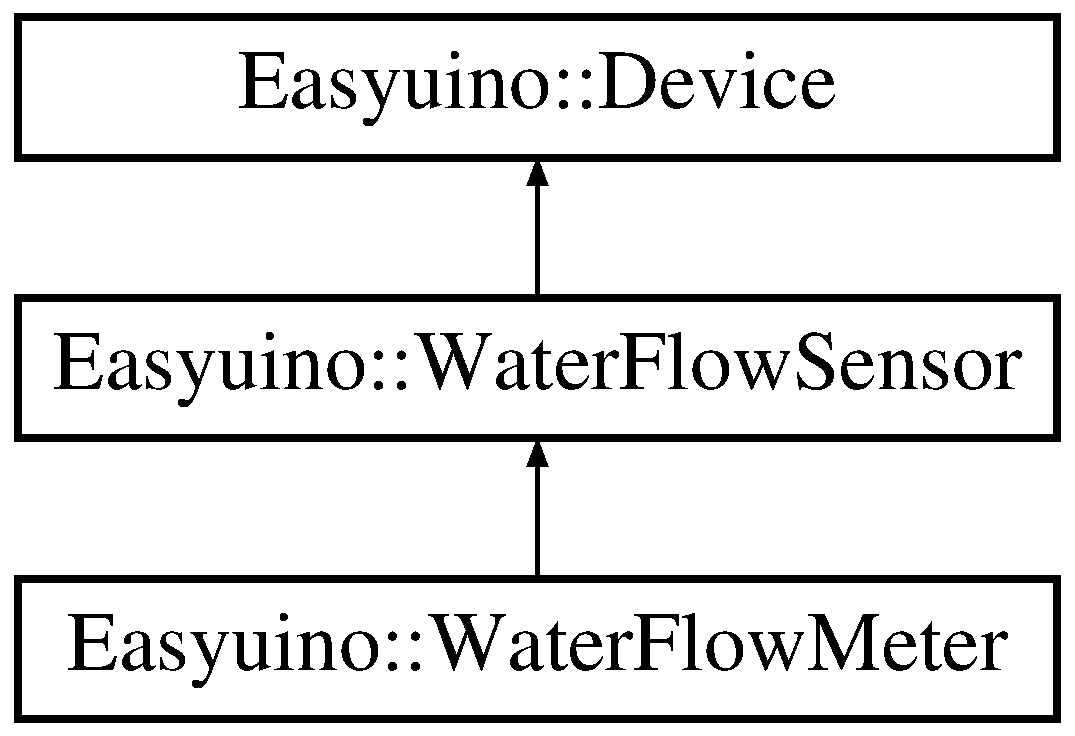
\includegraphics[height=3.000000cm]{class_easyuino_1_1_water_flow_meter}
\end{center}
\end{figure}
\subsection*{Public Member Functions}
\begin{DoxyCompactItemize}
\item 
\hyperlink{class_easyuino_1_1_water_flow_meter_a51374e5ffa6327028f4d5fe730083672}{Water\+Flow\+Meter} (IN uint8\+\_\+t sensor\+Pin, IN float sensor\+Calibration\+Factor)
\begin{DoxyCompactList}\small\item\em Constructor. \end{DoxyCompactList}\item 
\mbox{\Hypertarget{class_easyuino_1_1_water_flow_meter_ab9f6129be636d43c426eed5b5b42e088}\label{class_easyuino_1_1_water_flow_meter_ab9f6129be636d43c426eed5b5b42e088}} 
\hyperlink{class_easyuino_1_1_water_flow_meter_ab9f6129be636d43c426eed5b5b42e088}{$\sim$\+Water\+Flow\+Meter} ()
\begin{DoxyCompactList}\small\item\em Destructor. \end{DoxyCompactList}\item 
bool \hyperlink{class_easyuino_1_1_water_flow_meter_a400c25b10a7cde45c623805546d071cd}{begin} ()
\begin{DoxyCompactList}\small\item\em Used to put the device ready to receive requests. \end{DoxyCompactList}\item 
void \hyperlink{class_easyuino_1_1_water_flow_meter_a47024d4da9568e42743a875c08c33121}{end} ()
\begin{DoxyCompactList}\small\item\em Used to stop the device A\+PI. \end{DoxyCompactList}\item 
float \hyperlink{class_easyuino_1_1_water_flow_meter_ab8d3afb56987644486dcf6e17457269d}{get\+Flow\+Rate\+Liters\+Min} ()
\begin{DoxyCompactList}\small\item\em Returns the current flow rate that is passing through the flow meter. \end{DoxyCompactList}\end{DoxyCompactItemize}
\subsection*{Protected Member Functions}
\begin{DoxyCompactItemize}
\item 
void \hyperlink{class_easyuino_1_1_water_flow_meter_a9f9b39b7961175f027dad4fe75271569}{pulse\+Handler} (IN unsigned long call\+Timestamp)
\begin{DoxyCompactList}\small\item\em Called by the interruption I\+SR for each pulse. \end{DoxyCompactList}\end{DoxyCompactItemize}
\subsection*{Additional Inherited Members}


\subsection{Detailed Description}
\hyperlink{class_easyuino_1_1_water_flow_meter}{Water\+Flow\+Meter} A\+PI extends the \hyperlink{class_easyuino_1_1_water_flow_sensor}{Water\+Flow\+Sensor} A\+PI adding the possiblity to know how much water is flowing and how much have flown in total. 

\begin{DoxySeeAlso}{See also}
Limitation\+: This allows O\+N\+LY 1 instance of \hyperlink{class_easyuino_1_1_water_flow_meter}{Water\+Flow\+Meter} per sketch!! 

Devices Supported\+: Y\+F-\/\+D\+N40 

Devices Tested\+: Y\+F-\/\+D\+N40 
\end{DoxySeeAlso}


\subsection{Constructor \& Destructor Documentation}
\mbox{\Hypertarget{class_easyuino_1_1_water_flow_meter_a51374e5ffa6327028f4d5fe730083672}\label{class_easyuino_1_1_water_flow_meter_a51374e5ffa6327028f4d5fe730083672}} 
\index{Easyuino\+::\+Water\+Flow\+Meter@{Easyuino\+::\+Water\+Flow\+Meter}!Water\+Flow\+Meter@{Water\+Flow\+Meter}}
\index{Water\+Flow\+Meter@{Water\+Flow\+Meter}!Easyuino\+::\+Water\+Flow\+Meter@{Easyuino\+::\+Water\+Flow\+Meter}}
\subsubsection{\texorpdfstring{Water\+Flow\+Meter()}{WaterFlowMeter()}}
{\footnotesize\ttfamily Easyuino\+::\+Water\+Flow\+Meter\+::\+Water\+Flow\+Meter (\begin{DoxyParamCaption}\item[{IN uint8\+\_\+t}]{sensor\+Pin,  }\item[{IN float}]{sensor\+Calibration\+Factor }\end{DoxyParamCaption})}



Constructor. 


\begin{DoxyParams}{Parameters}
{\em sensor\+Pin} & Arduino pin connected to the sensor pulse pin \\
\hline
{\em sensor\+Calibration\+Factor} & Calibration factor that comes with the sensor specs, necessary for a good calculation of the flow rate and the total amount flowed (e.\+g\+: 0.\+2 in case of Y\+F-\/\+D\+N40) \\
\hline
\end{DoxyParams}


\subsection{Member Function Documentation}
\mbox{\Hypertarget{class_easyuino_1_1_water_flow_meter_a400c25b10a7cde45c623805546d071cd}\label{class_easyuino_1_1_water_flow_meter_a400c25b10a7cde45c623805546d071cd}} 
\index{Easyuino\+::\+Water\+Flow\+Meter@{Easyuino\+::\+Water\+Flow\+Meter}!begin@{begin}}
\index{begin@{begin}!Easyuino\+::\+Water\+Flow\+Meter@{Easyuino\+::\+Water\+Flow\+Meter}}
\subsubsection{\texorpdfstring{begin()}{begin()}}
{\footnotesize\ttfamily bool Easyuino\+::\+Water\+Flow\+Meter\+::begin (\begin{DoxyParamCaption}{ }\end{DoxyParamCaption})\hspace{0.3cm}{\ttfamily [virtual]}}



Used to put the device ready to receive requests. 

Normally this have some default behaviour some devices have other overload method with same name that receives other arguments to device customization. \begin{DoxyReturn}{Returns}
True\+: If the device was initialized. False\+: Otherwise. 
\end{DoxyReturn}


Implements \hyperlink{class_easyuino_1_1_device_a2e7bb2fec849719a9d9432b57cdb72ba}{Easyuino\+::\+Device}.

\mbox{\Hypertarget{class_easyuino_1_1_water_flow_meter_a47024d4da9568e42743a875c08c33121}\label{class_easyuino_1_1_water_flow_meter_a47024d4da9568e42743a875c08c33121}} 
\index{Easyuino\+::\+Water\+Flow\+Meter@{Easyuino\+::\+Water\+Flow\+Meter}!end@{end}}
\index{end@{end}!Easyuino\+::\+Water\+Flow\+Meter@{Easyuino\+::\+Water\+Flow\+Meter}}
\subsubsection{\texorpdfstring{end()}{end()}}
{\footnotesize\ttfamily void Easyuino\+::\+Water\+Flow\+Meter\+::end (\begin{DoxyParamCaption}{ }\end{DoxyParamCaption})\hspace{0.3cm}{\ttfamily [virtual]}}



Used to stop the device A\+PI. 

After this the the device will not process A\+PI requests. 

Implements \hyperlink{class_easyuino_1_1_device_ab31018ef64adc84aa2ea575b2297548f}{Easyuino\+::\+Device}.

\mbox{\Hypertarget{class_easyuino_1_1_water_flow_meter_ab8d3afb56987644486dcf6e17457269d}\label{class_easyuino_1_1_water_flow_meter_ab8d3afb56987644486dcf6e17457269d}} 
\index{Easyuino\+::\+Water\+Flow\+Meter@{Easyuino\+::\+Water\+Flow\+Meter}!get\+Flow\+Rate\+Liters\+Min@{get\+Flow\+Rate\+Liters\+Min}}
\index{get\+Flow\+Rate\+Liters\+Min@{get\+Flow\+Rate\+Liters\+Min}!Easyuino\+::\+Water\+Flow\+Meter@{Easyuino\+::\+Water\+Flow\+Meter}}
\subsubsection{\texorpdfstring{get\+Flow\+Rate\+Liters\+Min()}{getFlowRateLitersMin()}}
{\footnotesize\ttfamily float Easyuino\+::\+Water\+Flow\+Meter\+::get\+Flow\+Rate\+Liters\+Min (\begin{DoxyParamCaption}{ }\end{DoxyParamCaption})}



Returns the current flow rate that is passing through the flow meter. 

\begin{DoxyReturn}{Returns}
flow\+Rate (Liters/min) The current flow rate. 
\end{DoxyReturn}
\mbox{\Hypertarget{class_easyuino_1_1_water_flow_meter_a9f9b39b7961175f027dad4fe75271569}\label{class_easyuino_1_1_water_flow_meter_a9f9b39b7961175f027dad4fe75271569}} 
\index{Easyuino\+::\+Water\+Flow\+Meter@{Easyuino\+::\+Water\+Flow\+Meter}!pulse\+Handler@{pulse\+Handler}}
\index{pulse\+Handler@{pulse\+Handler}!Easyuino\+::\+Water\+Flow\+Meter@{Easyuino\+::\+Water\+Flow\+Meter}}
\subsubsection{\texorpdfstring{pulse\+Handler()}{pulseHandler()}}
{\footnotesize\ttfamily void Easyuino\+::\+Water\+Flow\+Meter\+::pulse\+Handler (\begin{DoxyParamCaption}\item[{IN unsigned long}]{call\+Timestamp }\end{DoxyParamCaption})\hspace{0.3cm}{\ttfamily [protected]}, {\ttfamily [virtual]}}



Called by the interruption I\+SR for each pulse. 



Reimplemented from \hyperlink{class_easyuino_1_1_water_flow_sensor_ab359b33262e324fa757de05a13f05141}{Easyuino\+::\+Water\+Flow\+Sensor}.



The documentation for this class was generated from the following file\+:\begin{DoxyCompactItemize}
\item 
src/Water\+Flow\+Meter.\+h\end{DoxyCompactItemize}

\hypertarget{class_easyuino_1_1_water_flow_sensor}{}\section{Easyuino\+:\+:Water\+Flow\+Sensor Class Reference}
\label{class_easyuino_1_1_water_flow_sensor}\index{Easyuino\+::\+Water\+Flow\+Sensor@{Easyuino\+::\+Water\+Flow\+Sensor}}
Inheritance diagram for Easyuino\+:\+:Water\+Flow\+Sensor\+:\begin{figure}[H]
\begin{center}
\leavevmode
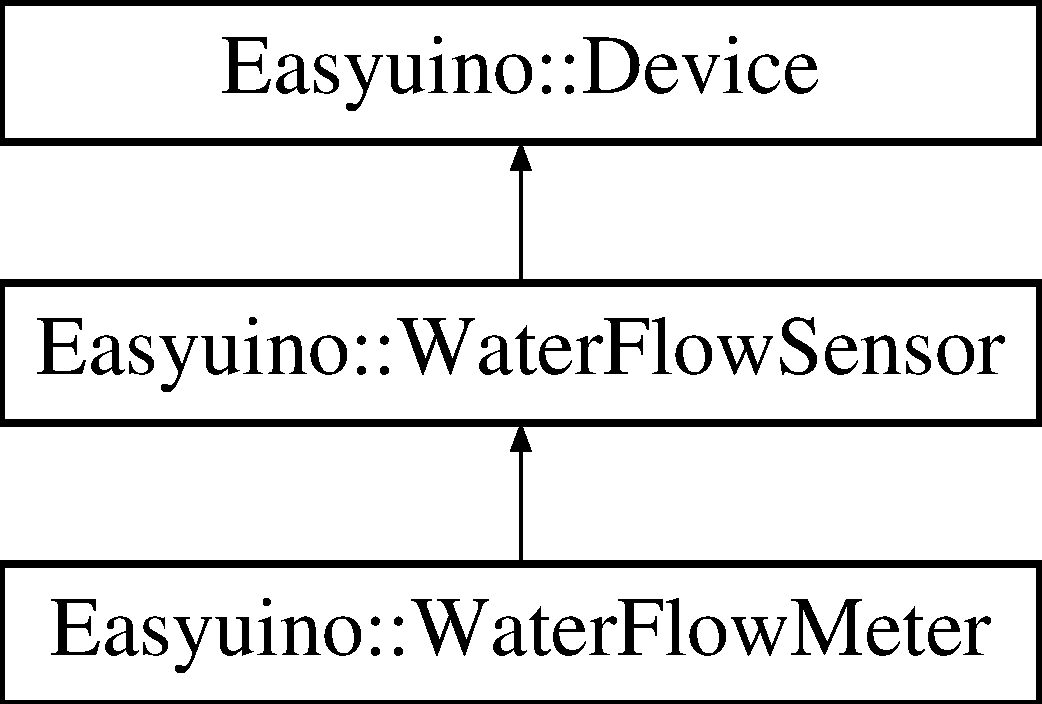
\includegraphics[height=3.000000cm]{class_easyuino_1_1_water_flow_sensor}
\end{center}
\end{figure}
\subsection*{Public Member Functions}
\begin{DoxyCompactItemize}
\item 
\mbox{\Hypertarget{class_easyuino_1_1_water_flow_sensor_acee82d1863cb2311e58210906d9fbfaa}\label{class_easyuino_1_1_water_flow_sensor_acee82d1863cb2311e58210906d9fbfaa}} 
{\bfseries Water\+Flow\+Sensor} (IN uint8\+\_\+t sensor\+Pin)
\item 
bool \hyperlink{class_easyuino_1_1_water_flow_sensor_a55dcab6c527b1e1951a1fff69efdb763}{begin} ()
\begin{DoxyCompactList}\small\item\em Used to put the device ready to receive requests. \end{DoxyCompactList}\item 
void \hyperlink{class_easyuino_1_1_water_flow_sensor_a7f31ac7735b049394d34cfbc37f17359}{end} ()
\begin{DoxyCompactList}\small\item\em Used to stop the device A\+PI. \end{DoxyCompactList}\item 
\mbox{\Hypertarget{class_easyuino_1_1_water_flow_sensor_a677d164cb17c56407c8102662b0c3cd4}\label{class_easyuino_1_1_water_flow_sensor_a677d164cb17c56407c8102662b0c3cd4}} 
virtual bool {\bfseries is\+Flowing} ()
\end{DoxyCompactItemize}
\subsection*{Protected Member Functions}
\begin{DoxyCompactItemize}
\item 
\mbox{\Hypertarget{class_easyuino_1_1_water_flow_sensor_adc2ba2c1888114b01719cfd6a659d59b}\label{class_easyuino_1_1_water_flow_sensor_adc2ba2c1888114b01719cfd6a659d59b}} 
void {\bfseries enable\+Pulse\+Counting} ()
\item 
\mbox{\Hypertarget{class_easyuino_1_1_water_flow_sensor_a66d275227c18329b38f33834b4682ff3}\label{class_easyuino_1_1_water_flow_sensor_a66d275227c18329b38f33834b4682ff3}} 
void {\bfseries disable\+Pulse\+Couning} ()
\end{DoxyCompactItemize}
\subsection*{Protected Attributes}
\begin{DoxyCompactItemize}
\item 
\mbox{\Hypertarget{class_easyuino_1_1_water_flow_sensor_a7efef15ef9da3a66bd40183c4ea908ff}\label{class_easyuino_1_1_water_flow_sensor_a7efef15ef9da3a66bd40183c4ea908ff}} 
uint8\+\_\+t {\bfseries \+\_\+sensor\+Pin}
\item 
\mbox{\Hypertarget{class_easyuino_1_1_water_flow_sensor_a8877c5e4a3ed8012341d416ce05fa93e}\label{class_easyuino_1_1_water_flow_sensor_a8877c5e4a3ed8012341d416ce05fa93e}} 
volatile uint32\+\_\+t {\bfseries \+\_\+pulse\+Counter}
\end{DoxyCompactItemize}


\subsection{Member Function Documentation}
\mbox{\Hypertarget{class_easyuino_1_1_water_flow_sensor_a55dcab6c527b1e1951a1fff69efdb763}\label{class_easyuino_1_1_water_flow_sensor_a55dcab6c527b1e1951a1fff69efdb763}} 
\index{Easyuino\+::\+Water\+Flow\+Sensor@{Easyuino\+::\+Water\+Flow\+Sensor}!begin@{begin}}
\index{begin@{begin}!Easyuino\+::\+Water\+Flow\+Sensor@{Easyuino\+::\+Water\+Flow\+Sensor}}
\subsubsection{\texorpdfstring{begin()}{begin()}}
{\footnotesize\ttfamily bool Easyuino\+::\+Water\+Flow\+Sensor\+::begin (\begin{DoxyParamCaption}{ }\end{DoxyParamCaption})\hspace{0.3cm}{\ttfamily [virtual]}}



Used to put the device ready to receive requests. 

Normally this have some default behaviour some devices have other overload method with same name that receives other arguments to device customization. \begin{DoxyReturn}{Returns}
True\+: If the device was initialized. False\+: Otherwise. 
\end{DoxyReturn}


Implements \hyperlink{class_easyuino_1_1_device_a2e7bb2fec849719a9d9432b57cdb72ba}{Easyuino\+::\+Device}.

\mbox{\Hypertarget{class_easyuino_1_1_water_flow_sensor_a7f31ac7735b049394d34cfbc37f17359}\label{class_easyuino_1_1_water_flow_sensor_a7f31ac7735b049394d34cfbc37f17359}} 
\index{Easyuino\+::\+Water\+Flow\+Sensor@{Easyuino\+::\+Water\+Flow\+Sensor}!end@{end}}
\index{end@{end}!Easyuino\+::\+Water\+Flow\+Sensor@{Easyuino\+::\+Water\+Flow\+Sensor}}
\subsubsection{\texorpdfstring{end()}{end()}}
{\footnotesize\ttfamily void Easyuino\+::\+Water\+Flow\+Sensor\+::end (\begin{DoxyParamCaption}{ }\end{DoxyParamCaption})\hspace{0.3cm}{\ttfamily [virtual]}}



Used to stop the device A\+PI. 

After this the the device will not process A\+PI requests. 

Implements \hyperlink{class_easyuino_1_1_device_ab31018ef64adc84aa2ea575b2297548f}{Easyuino\+::\+Device}.



The documentation for this class was generated from the following file\+:\begin{DoxyCompactItemize}
\item 
src/Water\+Flow\+Sensor.\+h\end{DoxyCompactItemize}

%--- End generated contents ---

% Index
\backmatter
\newpage
\phantomsection
\clearemptydoublepage
\addcontentsline{toc}{chapter}{Index}
\printindex

\end{document}
